\documentclass{beamer}

\usepackage[utf8]{inputenc}
\usepackage{default}
\usepackage{graphicx}
\usepackage{bbding}
\usepackage{color}

% TODO Learn what this does
% source
% http://tex.stackexchange.com/questions/15952/layout-of-multiple-lines-footnotes
% this is a way to adjust foot note so it can be cutted into multiple lines
\makeatletter
\renewcommand\@makefntext[1]{\tiny\rightskip=25em\hskip0em\@makefnmark#1}
\makeatother

\makeatletter
\newcommand*{\rom}[1]{\expandafter\@slowromancap\romannumeral #1@}
\makeatother


% shows how to change default (blue) colours in the default beamer theme
% found here: http://joerglenhard.wordpress.com/tag/latex/
\definecolor{WaterlooRed}{RGB}{145,11,46}
\setbeamercolor{title}{fg=WaterlooRed}
\setbeamercolor{frametitle}{fg=WaterlooRed}
\setbeamercolor{structure}{fg=WaterlooRed}

% adds logo in the footer
\logo{
\includegraphics[scale=.25]{img/csuow}}

\title[]{MicroFuge: A Middleware Approach to Providing Performance Isolation in Cloud Storage Systems}
\author[Akshay Singh, Xu Cui, Benjamin Cassell, Bernard Wong and Khuzaima Daudjee]{Akshay Singh, \textbf{Xu Cui}, Benjamin Cassell, Bernard Wong and Khuzaima Daudjee}
\institute{
\includegraphics[scale=0.25]{img/UniversityOfWaterloo_logo_vert_rgb.png}}
\date{{\tiny\today}}


% my macros
\newcommand{\myv}{\vspace{3 mm}}


\begin{document}

\begin{frame}
  \titlepage
\end{frame}


%% \begin{frame}
  %% \frametitle{Cloud Computing}

  %% Cloud computing allows us to share resources effectively at virtualized
  %% level, but at the same time we are sharing the physical resources and
  %% this comes at the cost of reduced isolation between tenants.


  %% \centering
  %% 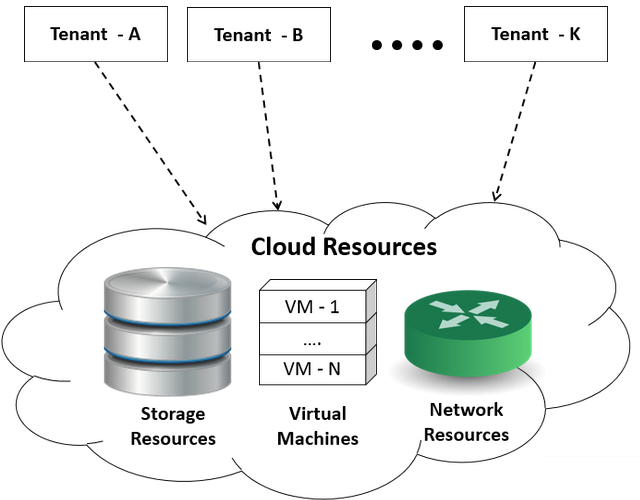
\includegraphics[scale=0.26]{img/icdcs1.png}

%% \end{frame}


\begin{frame}
  \frametitle{Storage Resources in Cloud Datacenters}
\vspace{-5 mm}
    \begin{itemize}
    \item Cloud computing allows sharing of resource at the cost of reduced isolation.
      \newline
    \item Storage systems are highly sensitive to performance interference.
      \newline
      \begin{itemize}
      \item Due to different access patterns - random vs. sequential.
      \end{itemize}
    \end{itemize}
\end{frame}

\begin{frame}
  \frametitle{A Typical Cloud Scenario}
  %% \vspace{5 mm}
  \begin{itemize}

  \item A HTTP request may require 35 database lookups.\footnote{Nathan Farrington and Alexey Andreyev, Facebook’s Data Center Network Architecture.}
    \begin{itemize}
      \myv
    \item  Response time can add up quickly.
    \end{itemize}
    \myv
  \item Studies\footnote{Akamai Technologies Inc. and Jupiter Research Inc.
    Akamai and Jupiter Research identify `4 seconds' as the new threshold of
    acceptability for retail web page response times.
    http\://www.akamai.com/html/about/press/releases/20
    06/press\_110606.html.}
    have shown that high latencies may drive customer away.
    \myv
  \item Predictable performance is desired.
    %% \centering
  \end{itemize}

\end{frame}

\begin{frame}
  \frametitle{Performance Isolation}
  \begin{itemize}
  \item Clients prefer to have the performance as if the resources are dedicated.
    \myv
  \item Possible solutions to performance isolation.
    \myv
    %% \vspace{-2.5 mm}
    \begin{itemize}
    \item Dedicated resources - costly.
      \myv
    \item Meet clients' response time requirements in the shared environment.
      \myv
    \item \(\text{Meeting response time requirement} \rightarrow \text{Performance Isolation.}\)
    \end{itemize}
  \end{itemize}
\end{frame}


\begin{frame}
  \frametitle{From a Customer's Point of View}
  \myv
  \begin{itemize}
  \item Clients want to differentiate their services.
    \myv
  \item Different requests have different response time requirements.
    \myv
  \item Capture the desired response time of requests with request deadlines.
  \end{itemize}
  \vspace{-5 mm}
  %% \begin{flushleft}
  \begin{figure}
    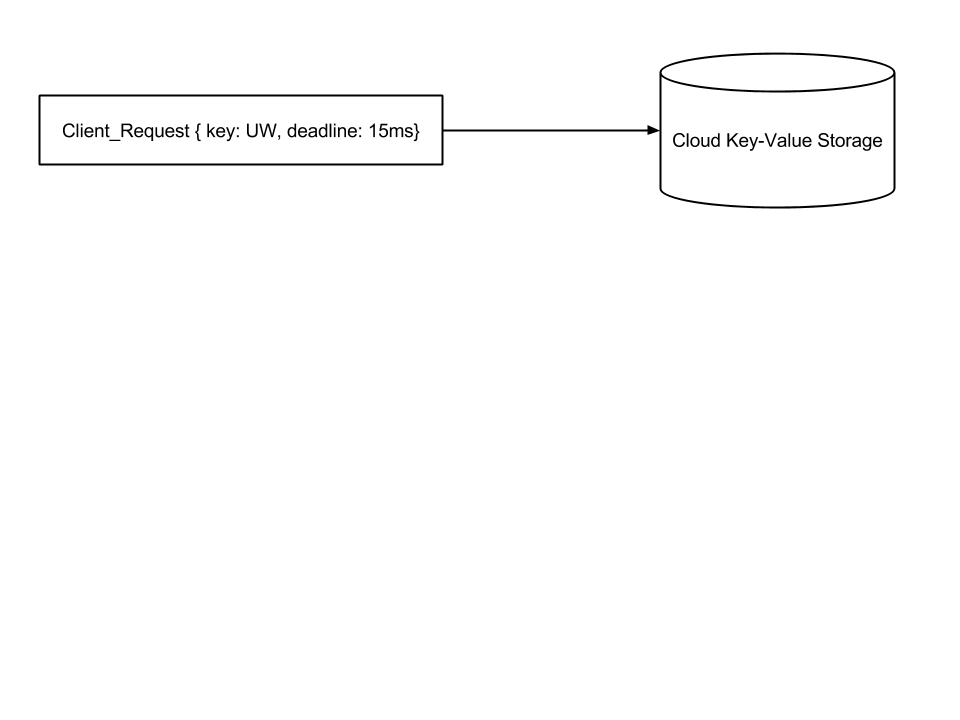
\includegraphics[scale=0.35]{img/Request_Deadline_Example.png}
  \end{figure}
  %% \end{flushleft}
\end{frame}

\begin{frame}
  \frametitle{Middleware Approach}
  \begin{itemize}
    \item Difficult to support numerous cloud storage systems.
      \myv
    \item Memcached - A popular middleware.
      \begin{itemize}
      \item Reduces response times.
      \item Deadline oblivious - doesn't distinguish different response time
        requirements.
      \end{itemize}
      \myv
    \item Similar approach to Memcached, use deadline-aware middleware to
      improve performance isolation.
  \end{itemize}
\end{frame}

\begin{frame}
  \frametitle{MicroFuge}
  \begin{itemize}
  \item A distributed caching and scheduling middleware that provides
    performance isolation.
    \myv
  \begin{itemize}
  \item \textbf{Deadline Cache (DLC)}
    \myv
      \begin{itemize}
      \item Performs deadline-aware evictions.
        \myv
      \end{itemize}
    \item \textbf{Deadline Scheduler (DLS)}
      \begin{itemize}
        \myv
      \item Performs deadline-aware scheduling.
        \myv
      \item {\textcolor[gray]{0.5} {Optionally performs admission control.}}
      \end{itemize}
  \end{itemize}
  \end{itemize}
\end{frame}

%% xcuiTODO: add the next slide to my latex sample/tutorial slides
%% \begin{frame}
  %% \frametitle{useful color text tutorial}
  %% \url{http://www-h.eng.cam.ac.uk/help/tpl/textprocessing/latex_advanced/colorandfonts.html}
  %% \\
  %% \myv
  %% \definecolor{gold}{rgb}{0.85,.66,0}
  %% This is in \textcolor{red}{red} and this box is \colorbox{gold}{gold}.
  %% Text color can be set using RGB values
  %% (\textcolor[rgb]{0,1,0}{like so}), or \textcolor[gray]{0.2}{shades}
  %% \textcolor[gray]{0.5}{of} \textcolor[gray]{0.8}{grey}.
%% \end{frame}

%% \begin{frame}
  %% \frametitle{Agenda}
  %% \begin{itemize}
  %% \item[\Checkmark] Background and Motivation
  %% \item MicroFuge
    %% \begin{itemize}
    %% \item Deadline Cache
    %% \item Deadline Scheduler
    %% \end{itemize}
  %% \item Evaluation
  %% \item Conclusion
  %% \end{itemize}
%% \end{frame}

\begin{frame}
  \frametitle{MicroFuge Overview (1)}
  \vspace{-10 mm}
  \begin{center}
  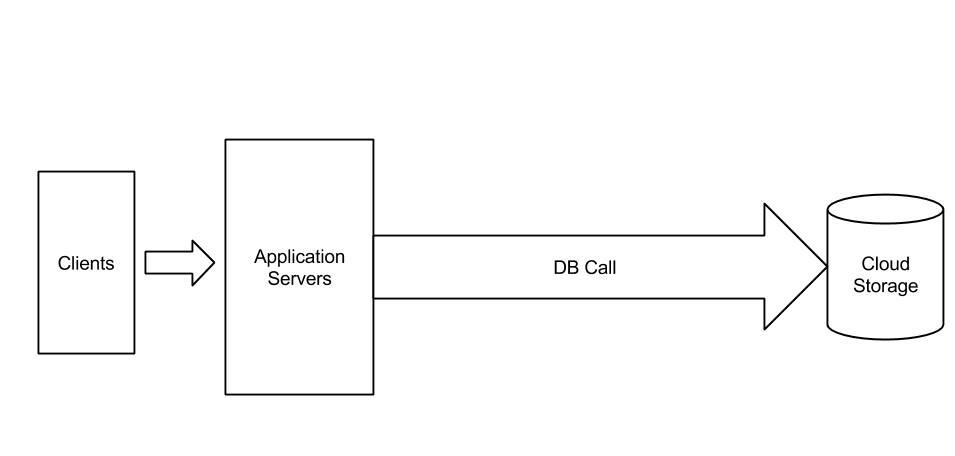
\includegraphics[scale=0.32]{img/MF_FULL_NEW_1.png}
  \end{center}
\end{frame}

\begin{frame}
  \frametitle{MicroFuge Overview (2)}
  \vspace{-10 mm}
  \begin{center}
  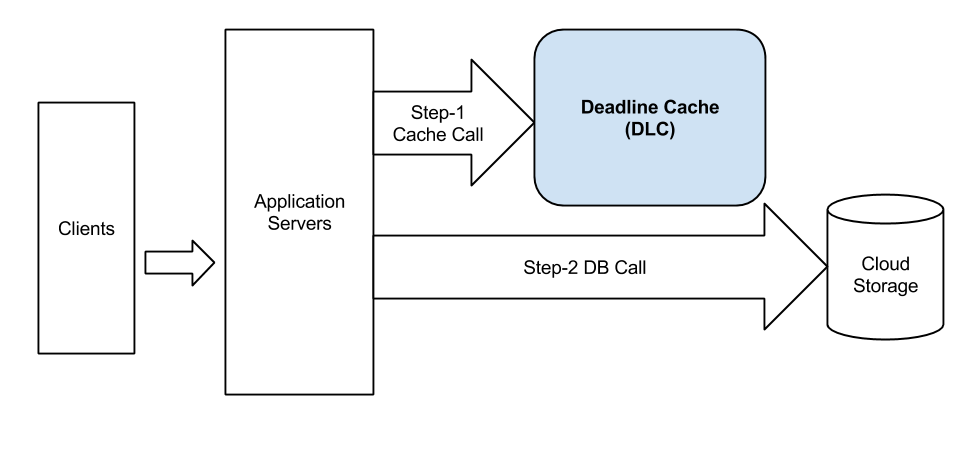
\includegraphics[scale=0.32]{img/MF_FULL_NEW_2.png}
  \end{center}
\end{frame}

\begin{frame}
  \frametitle{MicroFuge Overview (3)}
  \vspace{-10 mm}
  \begin{center}
  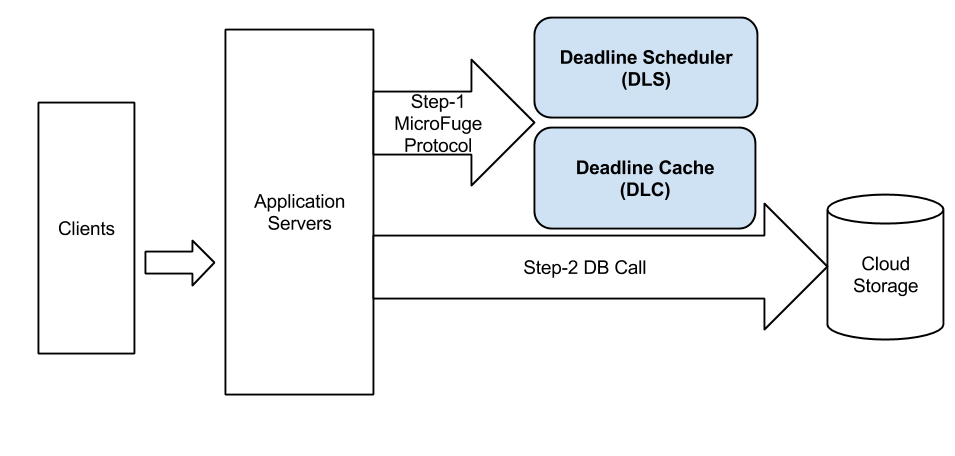
\includegraphics[scale=0.32]{img/MF_FULL_NEW_3.png}
  \end{center}
\end{frame}



\begin{frame}
  \frametitle{Contributions of MicroFuge}
  \vspace{-10 mm}
  \begin{itemize}
  \item \textbf{Deadline Cache (DLC)}
    \myv
    \begin{itemize}
    \item Performance modelling of the underlying storage system.
      \myv
    \item Use multiple LRU queues for deadline-aware eviction.
    \end{itemize}
    \myv
  \item \textbf{Deadline Scheduler (DLS)}
    \begin{itemize}
      \myv
    \item Performance modelling of the underlying storage system.
      \myv
    \item Deadline-aware scheduling.
      \myv
    \item \textcolor[gray]{0.5} {Admission control}.
    \end{itemize}
  \end{itemize}
\end {frame}



\begin{frame}
  \frametitle{MicroFuge at a Glance}
  \begin{itemize}
  \item Middleware for popular key-value storage.
    \myv
  \item A modified version of the CRUD operation interface.
    %% \centering
  \end{itemize}
  \begin{figure}
    %% \begin{flushleft}
\vspace{-5 mm}
  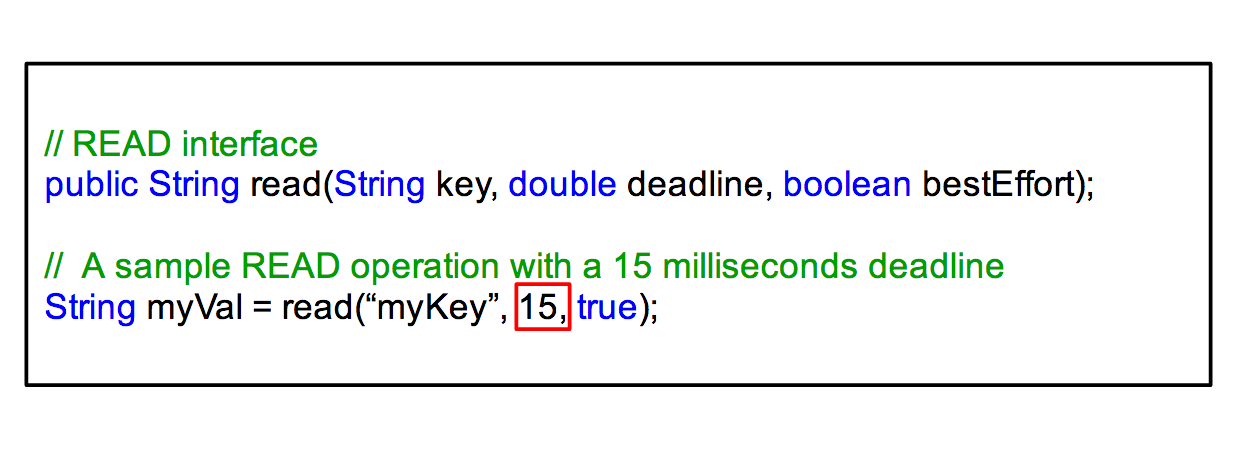
\includegraphics[scale=0.25]{img/MicroFuge_protocol.png}
  \caption{MicroFuge \textit{read} operation interface.}
    %% \end{flushleft}
  \end{figure}
\end{frame}

\begin{frame}
  \frametitle{Deadline Cache (DLC) - Components}
  \begin{figure}
    \begin{center}
      \centerline{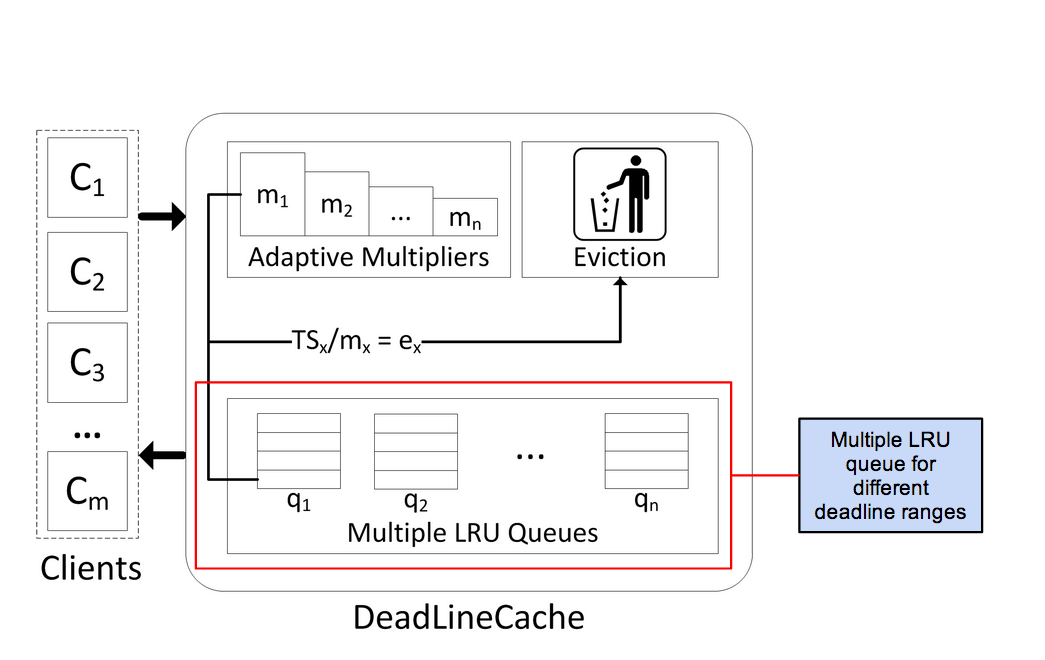
\includegraphics[scale=0.35]{img/DLC_ARC_1.png}}
    \end{center}
  \end{figure}
\end{frame}


\begin{frame}
  \frametitle{Deadline Cache (DLC) - Components}
  \begin{figure}
    \begin{center}
      \centerline{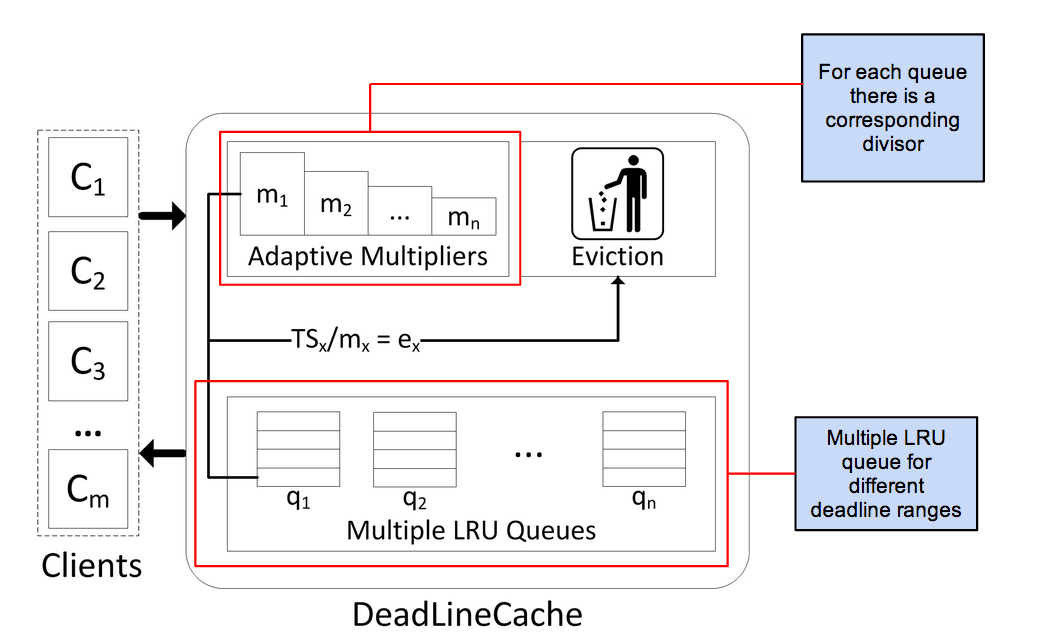
\includegraphics[scale=0.35]{img/DLC_ARC_2.png}}
    \end{center}
  \end{figure}
\end{frame}


\begin{frame}
  \frametitle{Deadline Cache (DLC) - Components}
  \begin{figure}
    \begin{center}
      \centerline{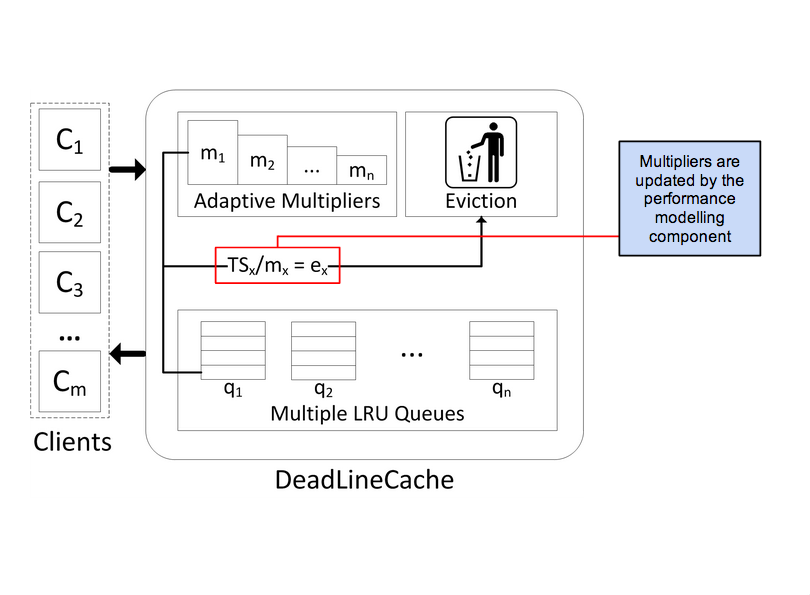
\includegraphics[scale=0.35]{img/DLC_ARC_3.png}}
    \end{center}
  \end{figure}
\end{frame}

\begin{frame}
  \frametitle{DLC - An Cache Eviction Example (1)}
  \begin{figure}
    \begin{center}
      \centerline{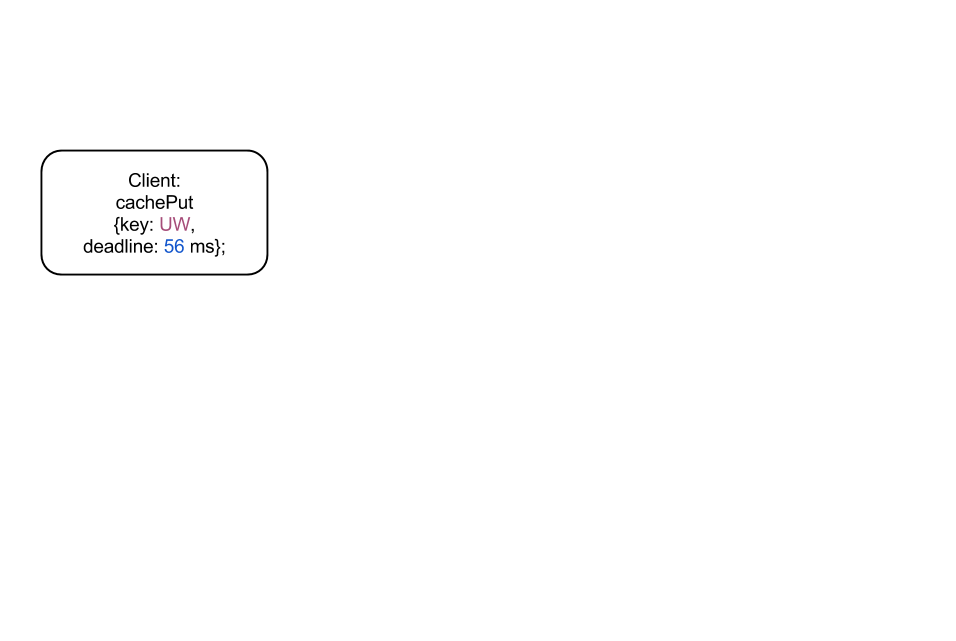
\includegraphics[scale=0.33]{img/DLC_V5_1.png}}
    \end{center}
  \end{figure}
\end{frame}


\begin{frame}
  \frametitle{DLC - An Cache Eviction Example (2)}
  \begin{figure}
    \begin{center}
      \centerline{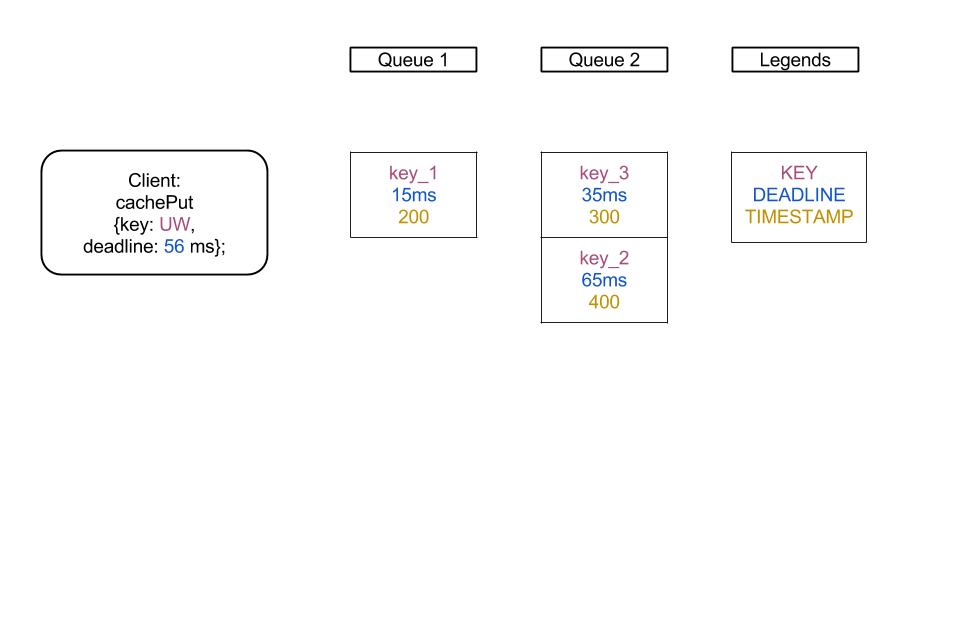
\includegraphics[scale=0.33]{img/DLC_V5_2.png}}
    \end{center}
  \end{figure}
\end{frame}

\begin{frame}
  \frametitle{DLC - An Cache Eviction Example (3)}
  \begin{figure}
    \begin{center}
      \centerline{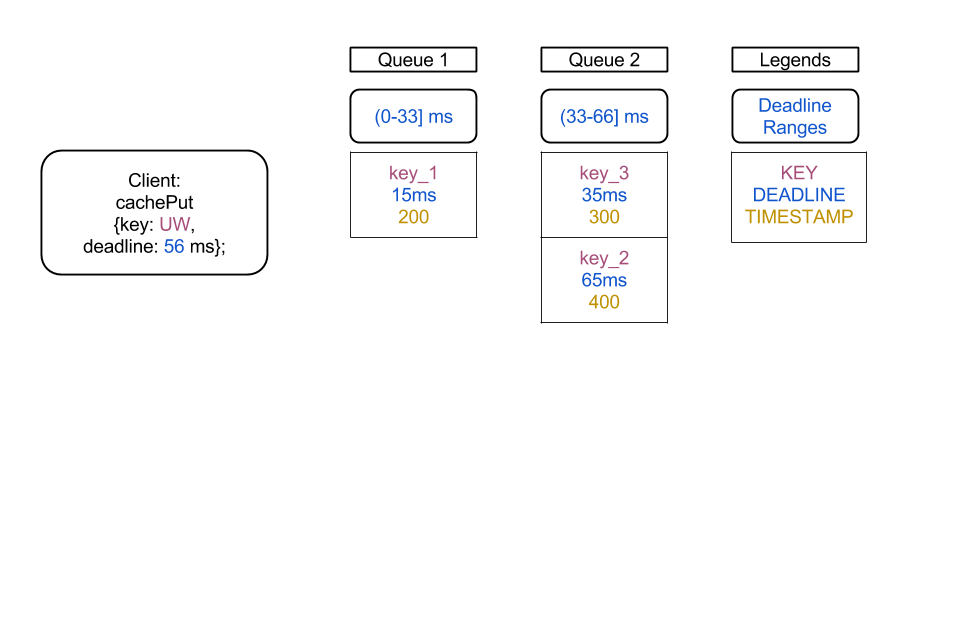
\includegraphics[scale=0.33]{img/DLC_V5_3.png}}
    \end{center}
  \end{figure}
\end{frame}

\begin{frame}
  \frametitle{DLC - An Cache Eviction Example (4)}
  \begin{figure}
    \begin{center}
      \centerline{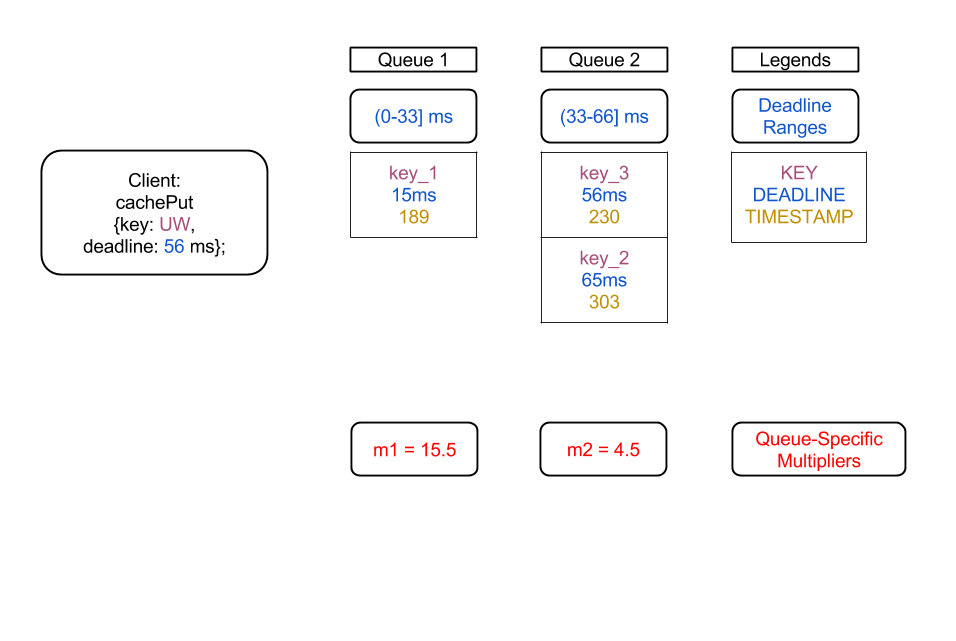
\includegraphics[scale=0.33]{img/DLC_V5_4.png}}
    \end{center}
  \end{figure}
\end{frame}


\begin{frame}
  \frametitle{DLC - An Cache Eviction Example (5)}
  \begin{figure}
    \begin{center}
      \centerline{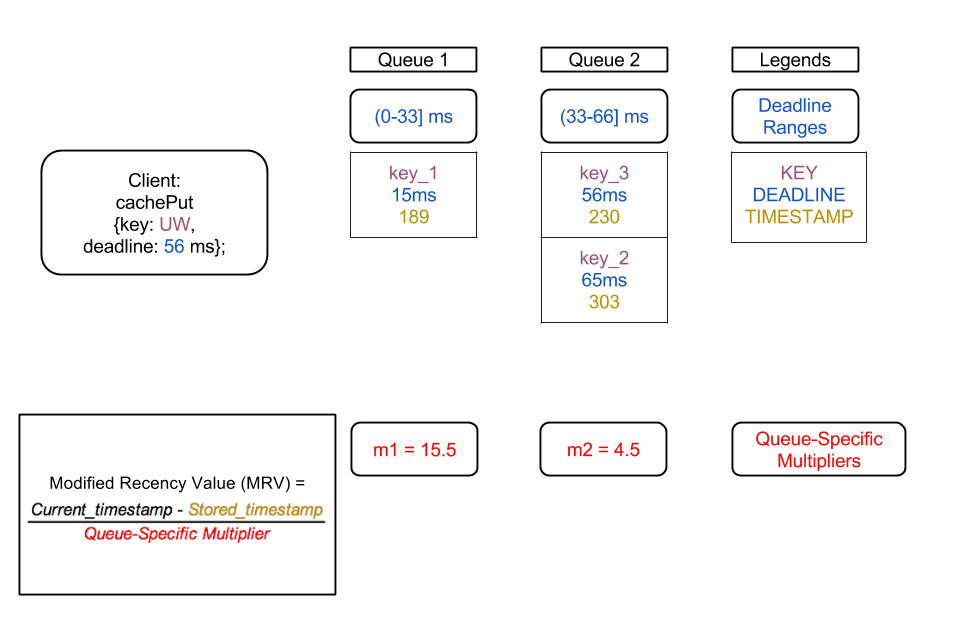
\includegraphics[scale=0.33]{img/DLC_V5_5.png}}
    \end{center}
  \end{figure}
\end{frame}

\begin{frame}
  \frametitle{DLC - An Cache Eviction Example (6)}
  \begin{figure}
    \begin{center}
      \centerline{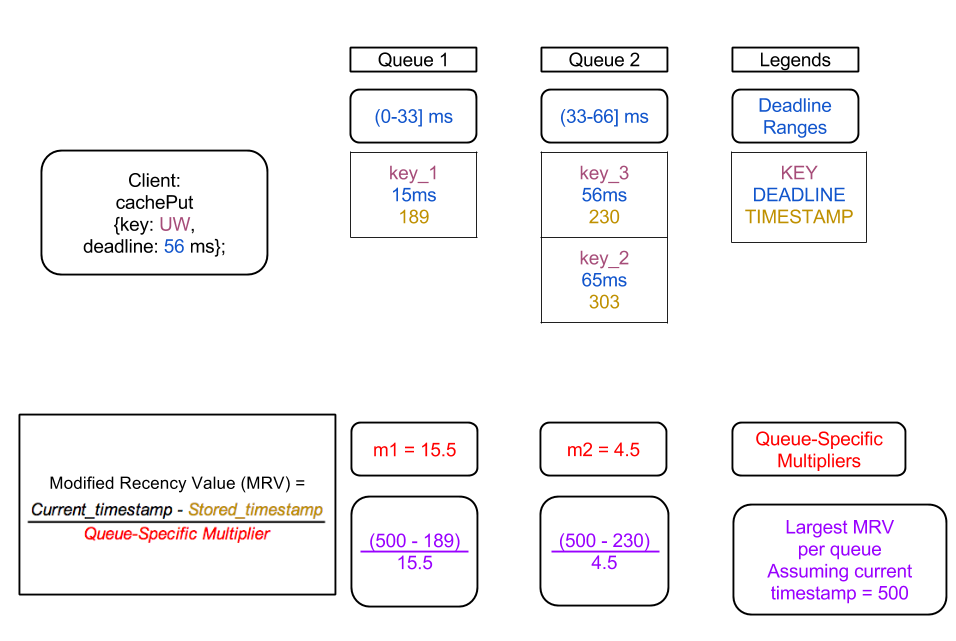
\includegraphics[scale=0.33]{img/DLC_V5_6.png}}
    \end{center}
  \end{figure}
\end{frame}

\begin{frame}
  \frametitle{DLC - An Cache Eviction Example (7)}
  \begin{figure}
    \begin{center}
      \centerline{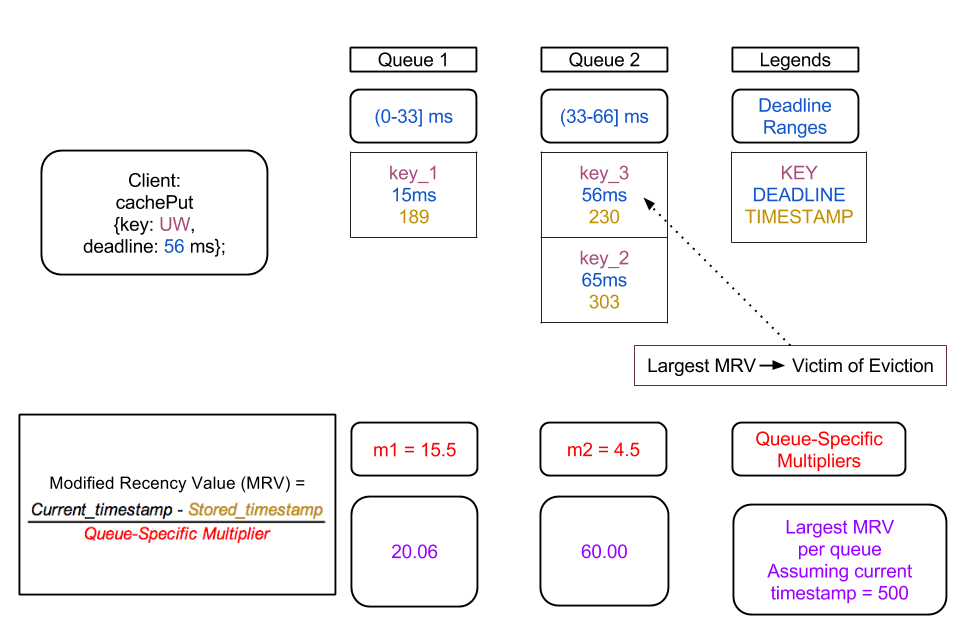
\includegraphics[scale=0.33]{img/DLC_V5_7.png}}
    \end{center}
  \end{figure}
\end{frame}

\begin{frame}
  \frametitle{DLC - An Cache Eviction Example (8)}
  \begin{figure}
    \begin{center}
      \centerline{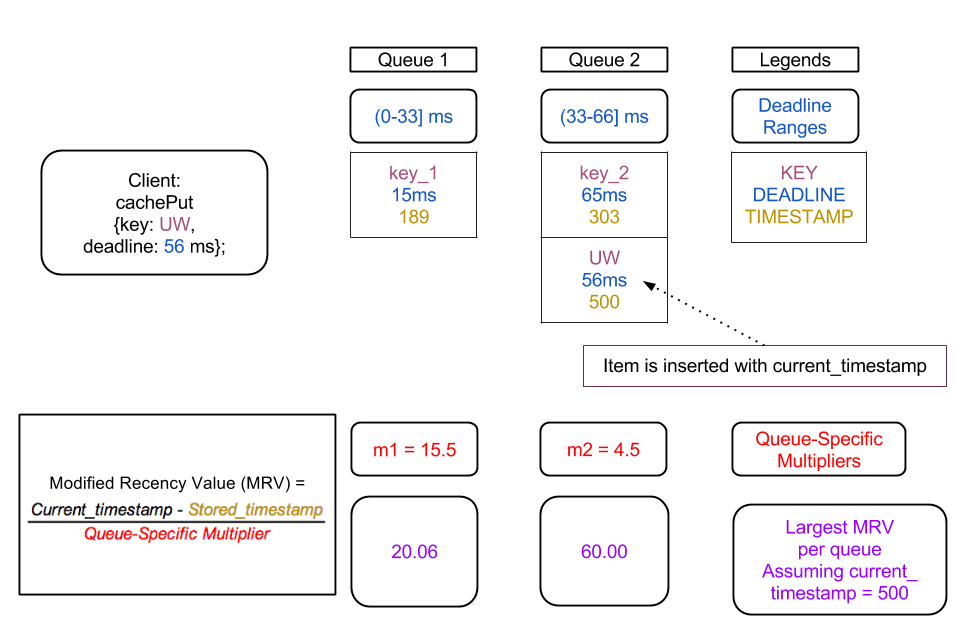
\includegraphics[scale=0.33]{img/DLC_V5_8.png}}
    \end{center}
  \end{figure}
\end{frame}

\begin{frame}
  \frametitle{DLC - An Cache Eviction Example (9)}
  \begin{figure}
    \begin{center}
      \centerline{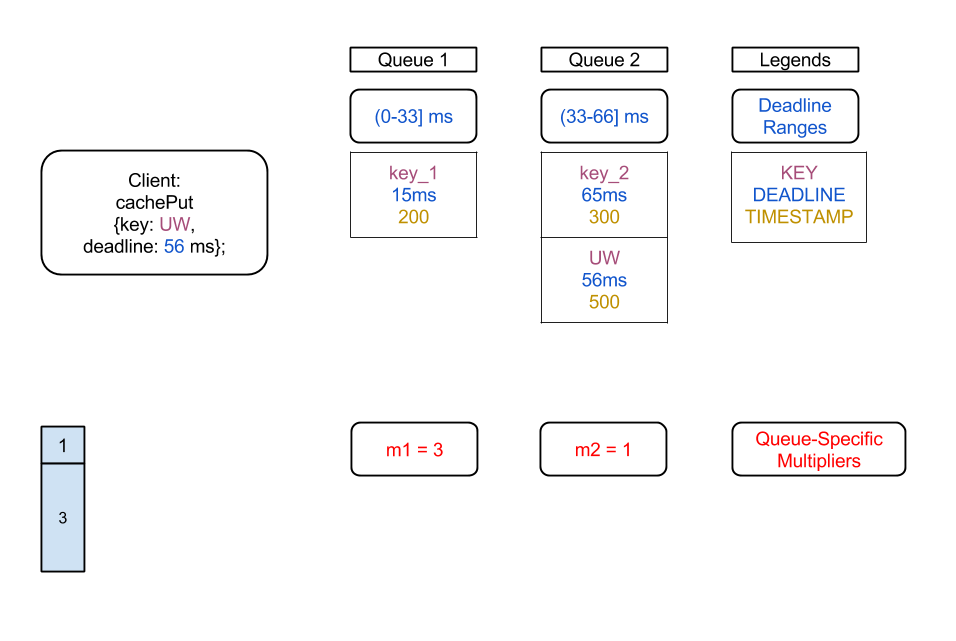
\includegraphics[scale=0.33]{img/DLC_V5_9.png}}
    \end{center}
  \end{figure}
\end{frame}

\begin{frame}
  \frametitle{DLC - An Cache Eviction Example (10)}
  \begin{figure}
    \begin{center}
      \centerline{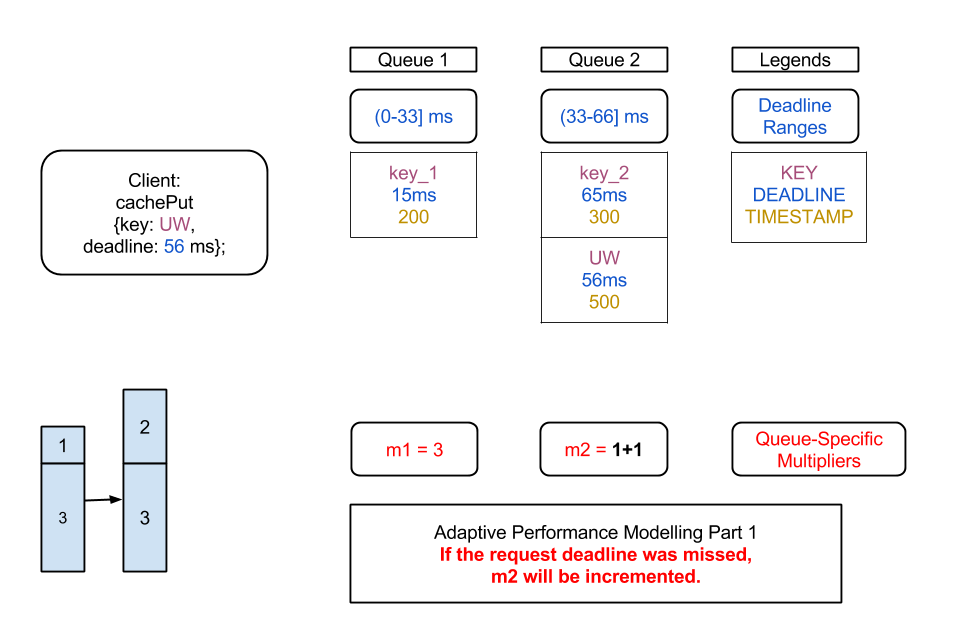
\includegraphics[scale=0.33]{img/DLC_V5_10.png}}
    \end{center}
  \end{figure}
\end{frame}

\begin{frame}
  \frametitle{DLC - An Cache Eviction Example (11)}
  \begin{figure}
    \begin{center}
      \centerline{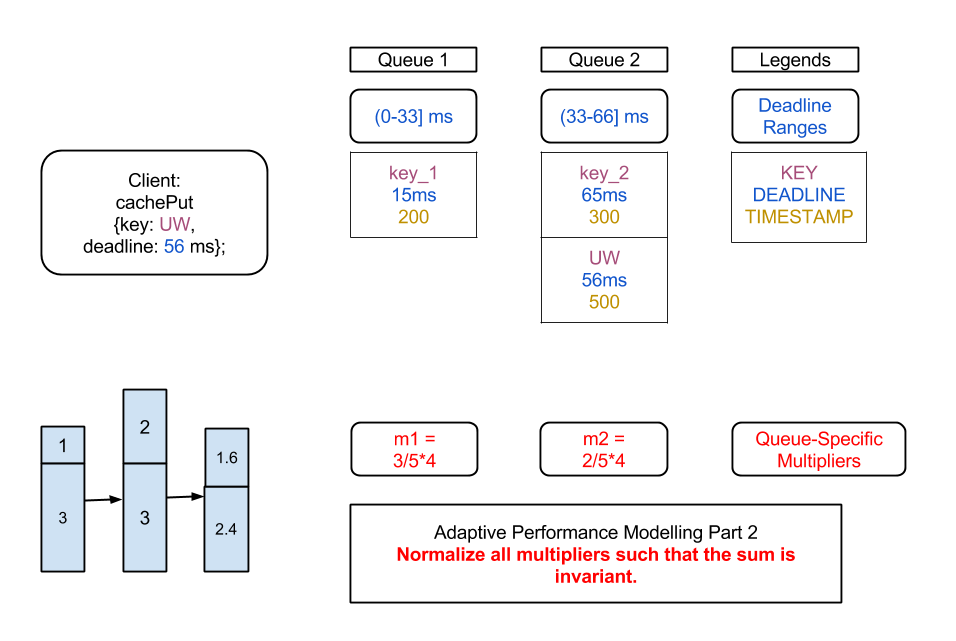
\includegraphics[scale=0.33]{img/DLC_V5_11.png}}
    \end{center}
  \end{figure}
\end{frame}


\begin{frame}
  \frametitle{DLC - Advantages}
  \vspace{-15 mm}
  \begin{itemize}
  \item Deadline-aware - favour items with shorter deadlines in terms
    of memory allocation. \myv
  \item LRU - favour items which are accessed more frequently. \myv
  \item Adaptiveness - favour items which are more likely to miss their
    deadlines.  \myv
  \item \textbf{DLC} - combines all three to achieve adaptive deadline-aware caching.
  \end{itemize}
\end{frame}


\begin{frame}
  \frametitle{Deadline Scheduler (DLS) High-level Architecture}
  \begin{itemize}
  \item Each scheduler is responsible for
    controlling the access to a single data-server.
  \end{itemize}
  \begin{figure}
    \begin{center}
      \centerline{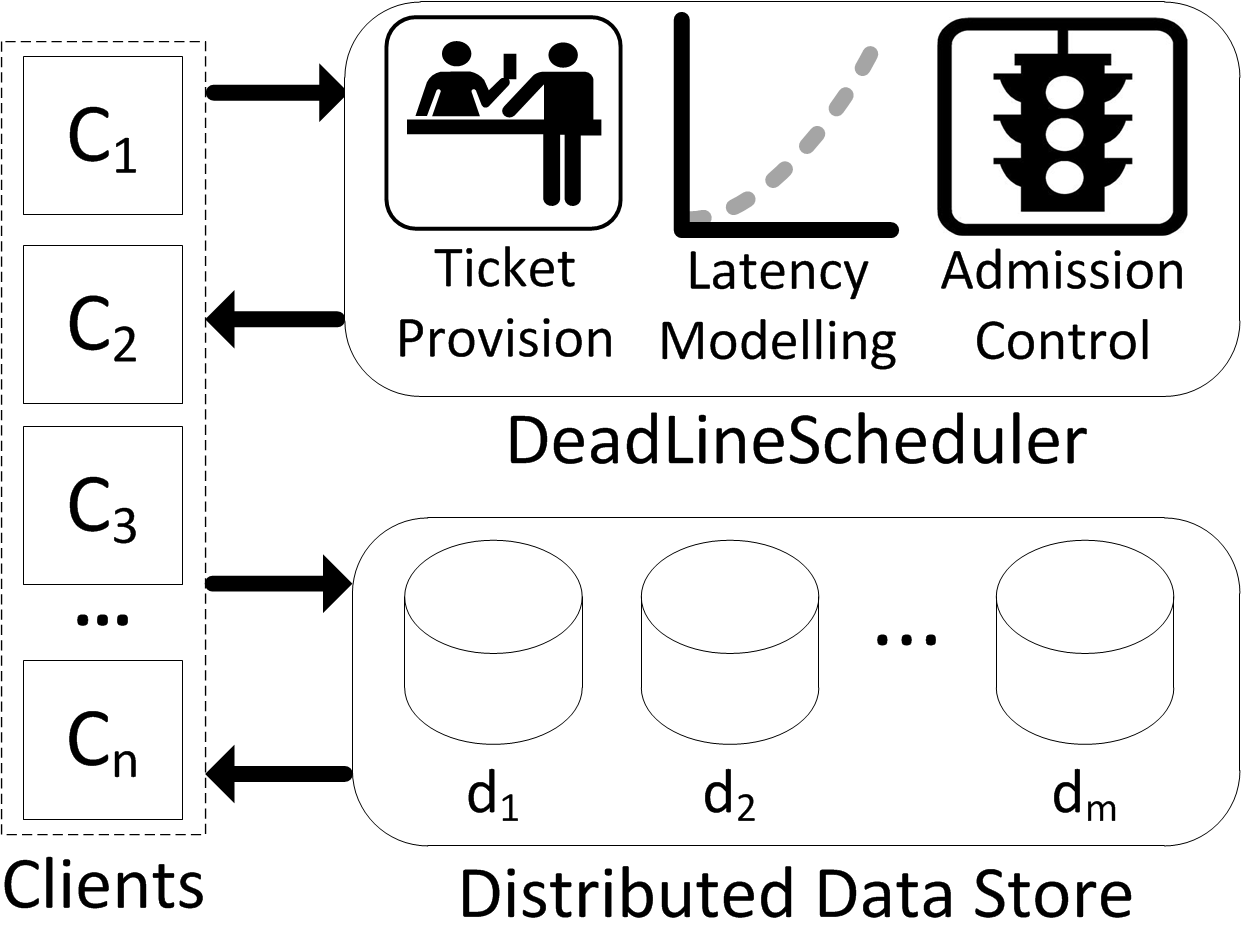
\includegraphics[scale=0.90]{img/DLS.png}}
    \end{center}
  \end{figure}
\end{frame}

\begin{frame}
  \frametitle{DLS - An Example Setup}
  \begin{itemize}
  \item Each key-value pair is replicated three times.
    \newline

  \end{itemize}
  \begin{figure}
    \begin{center}
      \centerline{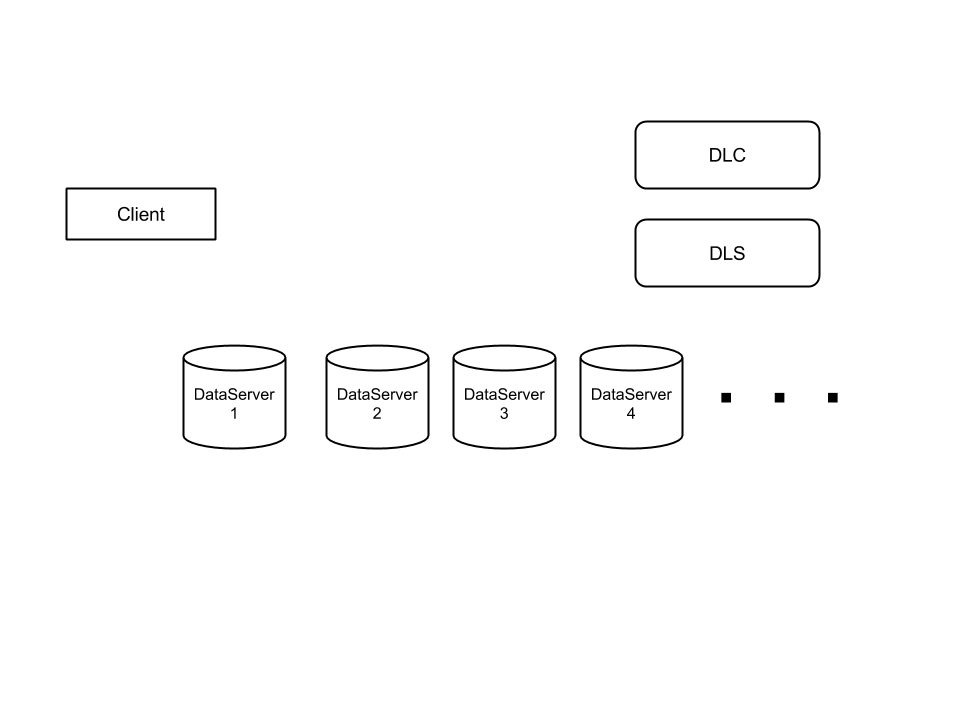
\includegraphics[scale=0.40]{img/DLS_Example1.png}}
    \end{center}
  \end{figure}

\end{frame}


\begin{frame}
  \frametitle{DLS - An Example (1)}
  \begin{itemize}
  \item The client wants to perform a simple value lookup for the key UW.
  \end{itemize}
  \begin{figure}
    \begin{center}
      \centerline{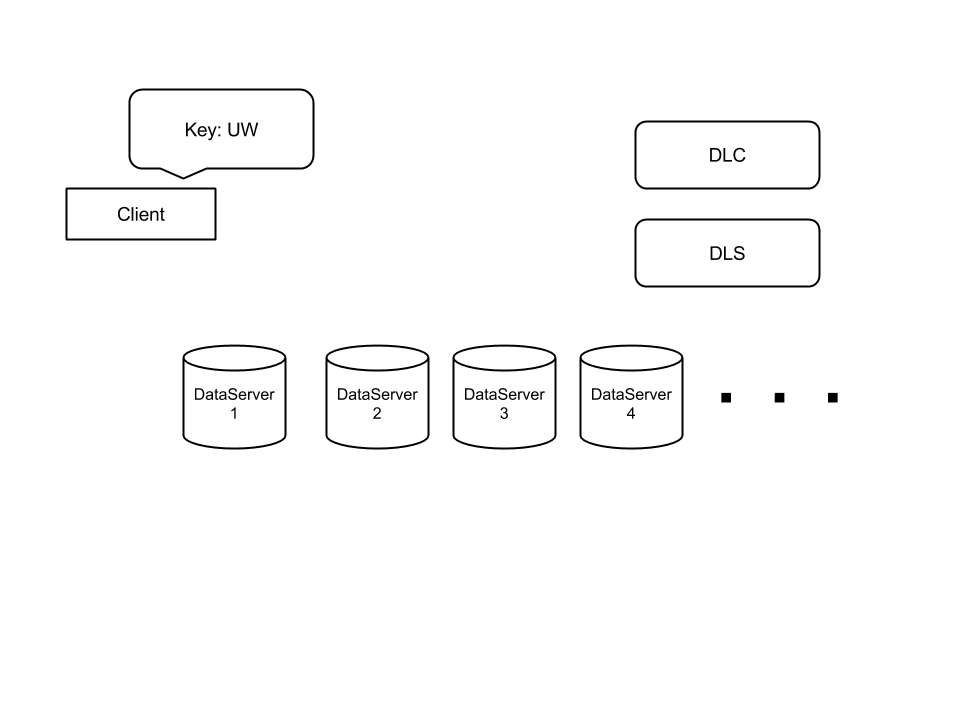
\includegraphics[scale=0.40]{img/DLS_Example2.png}}
    \end{center}
  \end{figure}
\end{frame}


\begin{frame}
  \frametitle{DLS - An Example (2)}
  \begin{itemize}
  \item The client begins by issuing a cache lookup to DLC.
\newline
  \end{itemize}
  \begin{figure}
    \begin{center}
      \centerline{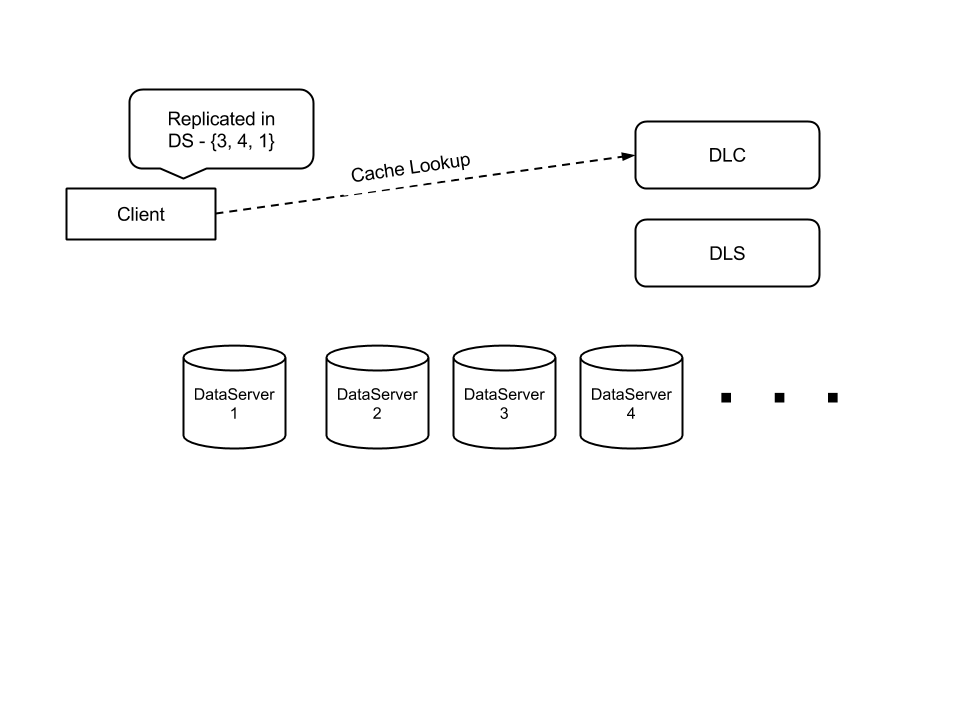
\includegraphics[scale=0.40]{img/DLS_Example3.png}}
    \end{center}
  \end{figure}


\end{frame}

\begin{frame}
  \frametitle{DLS - An Example (3)}
  \begin{itemize}
  \item Issue ticket \textit{get requests} concurrently.
\newline
  \end{itemize}
  \begin{figure}
    \begin{center}
      \centerline{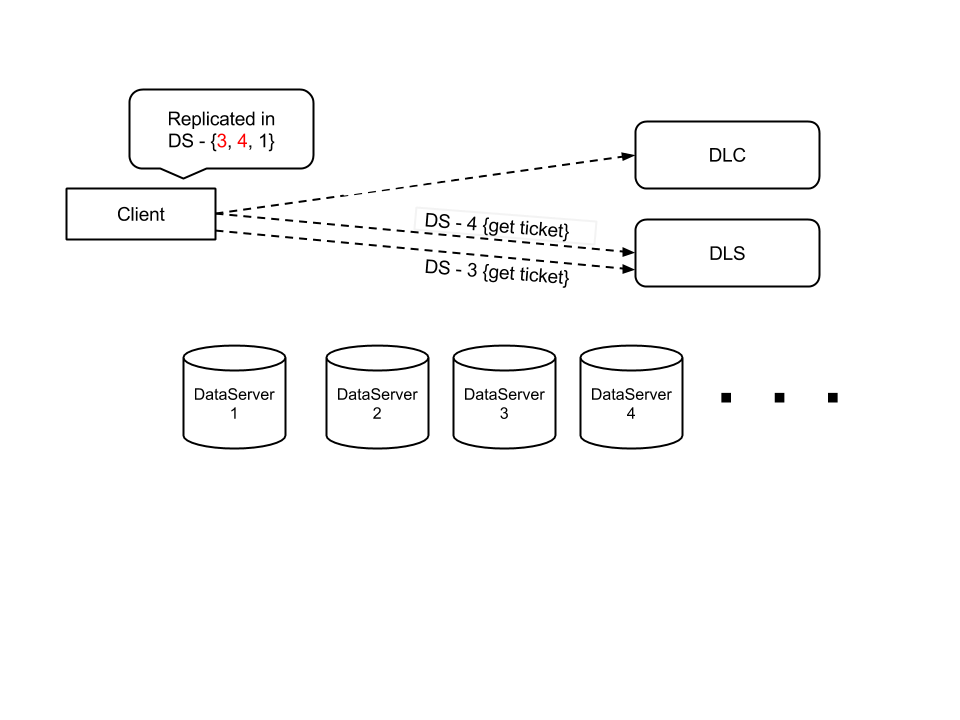
\includegraphics[scale=0.40]{img/DLS_Example4.png}}
    \end{center}
  \end{figure}

\end{frame}

\begin{frame}
  \frametitle{DLS - An Example (4)}
  \begin{itemize}
  \item If the item is not in the cache, the client waits for DLS to
    return the tickets.
  \end{itemize}
  \begin{figure}
    \begin{center}
      \centerline{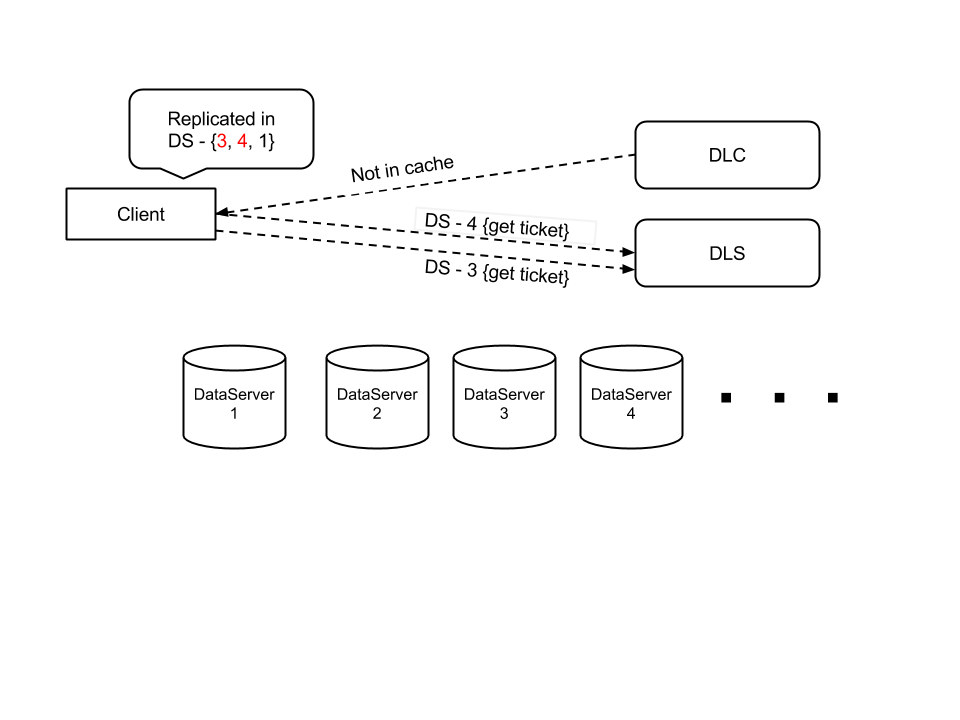
\includegraphics[scale=0.40]{img/DLS_Example5.png}}
    \end{center}
  \end{figure}
\end{frame}


\begin{frame}
  \frametitle{DLS - An Example (5)}
  \begin{itemize}
  \item When the tickets are sent back to the client, the client will pick
    the DLS server which responds the first.
  \end{itemize}
  \begin{figure}
    \begin{center}
      \centerline{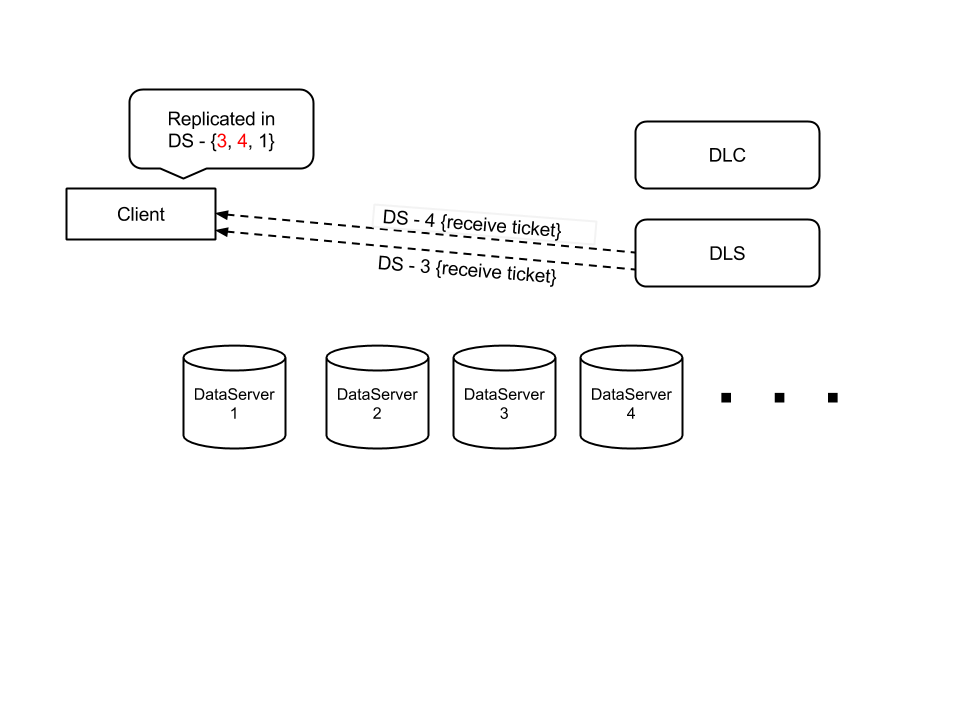
\includegraphics[scale=0.40]{img/DLS_Example6.png}}
    \end{center}
  \end{figure}
\end{frame}

\begin{frame}
  \frametitle{DLS - An Example (6)}
  \begin{itemize}
  \item The client makes a blocking call to the selected DLS and waits for
    its turn to access the data server.
  \end{itemize}
  \begin{figure}
    \begin{center}
      \centerline{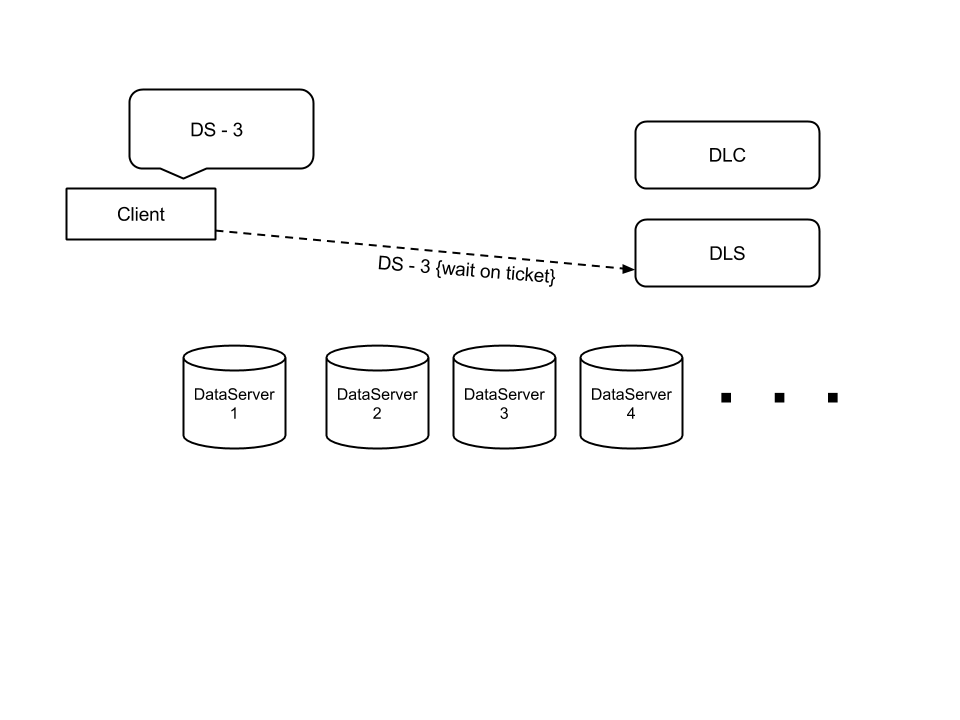
\includegraphics[scale=0.40]{img/DLS_Example7.png}}
    \end{center}
  \end{figure}
\end{frame}

\begin{frame}
  \frametitle{DLS - An Example (7)}
  \begin{itemize}
  \item Let's zoom in to look at the state of DLS's pending queue.
    \newline
    \newline
  \end{itemize}
  \begin{figure}
    \begin{center}
      \centerline{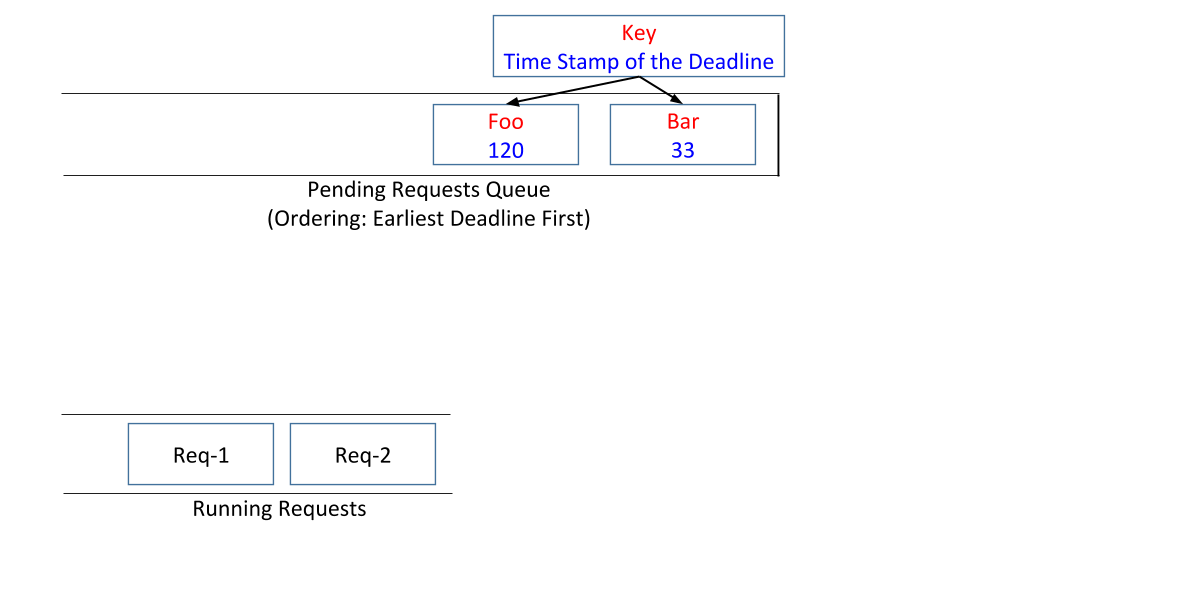
\includegraphics[scale=0.33]{img/DLS_Example8_1.png}}
    \end{center}
  \end{figure}
\end{frame}

\begin{frame}
  \frametitle{DLS - An Example (8)}
  \begin{itemize}
  \item The new item is inserted according to earliest deadline first ordering.
    \newline
  \end{itemize}
  \begin{figure}
    \begin{center}
      \centerline{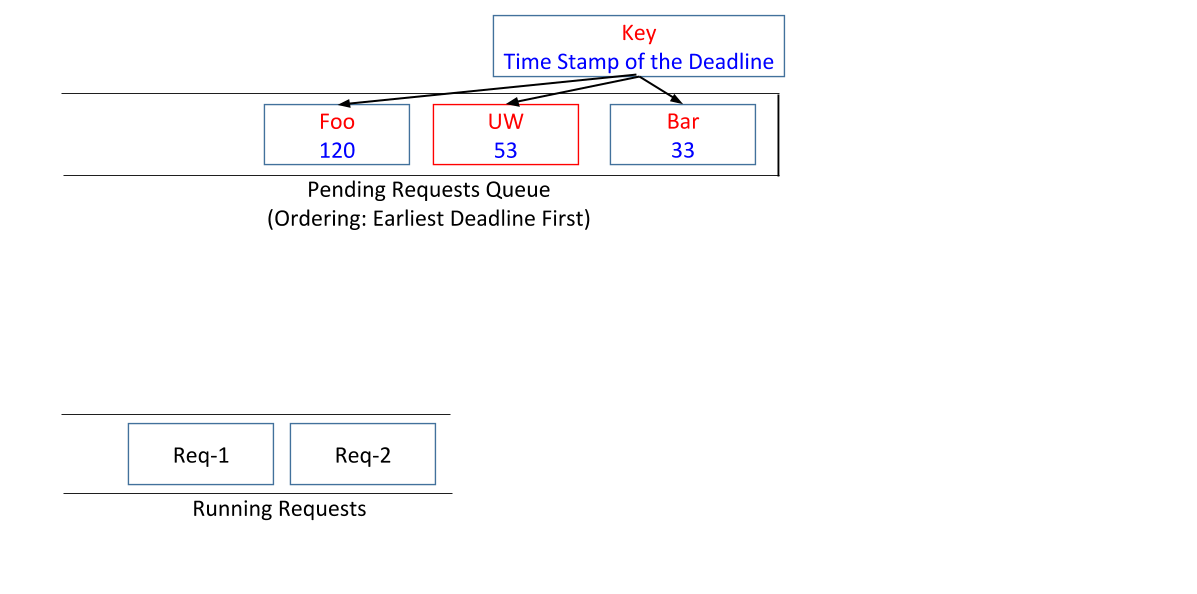
\includegraphics[scale=0.33]{img/DLS_Example8_2.png}}
    \end{center}
  \end{figure}
\end{frame}


\begin{frame}
  \frametitle{DLS - An Example (9)}
  \begin{itemize}
  \item Let's assume one of the running requests just completed.
    \newline
    \newline
  \end{itemize}
  \begin{figure}
    \begin{center}
      \centerline{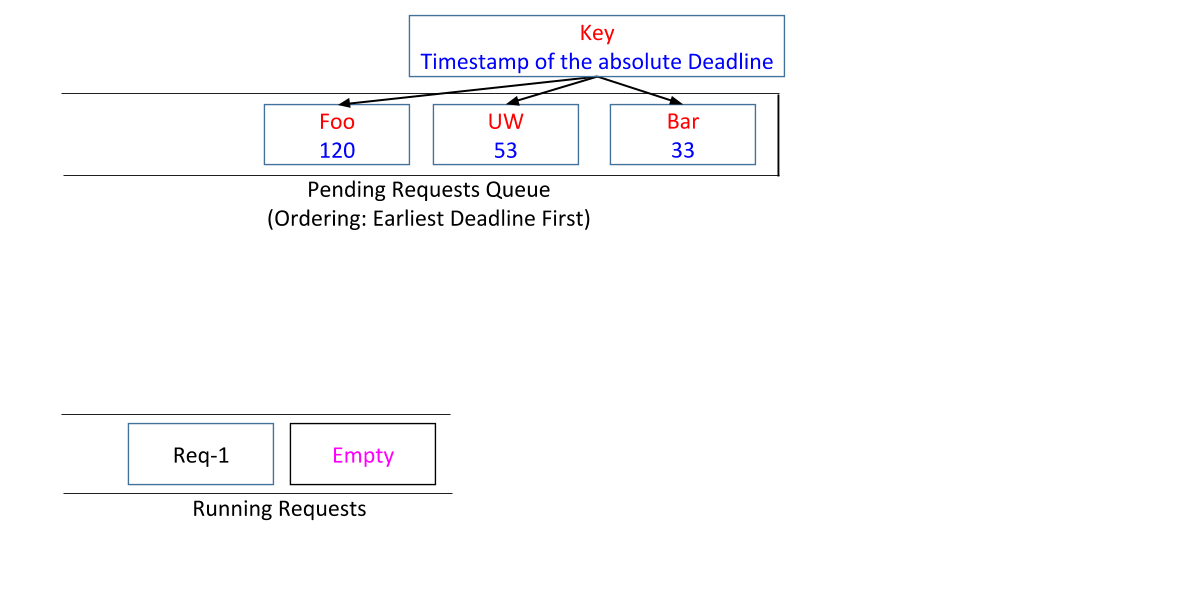
\includegraphics[scale=0.33]{img/DLS_Example8_3.png}}
    \end{center}
  \end{figure}
\end{frame}

\begin{frame}
  \frametitle{DLS - An Example (10)}
  \begin{itemize}
  \item DLS may increase the request's deadline and insert the request back
    into the queue if the deadline can not be met.
    \newline
  \end{itemize}
  \begin{figure}
    \begin{center}
      \centerline{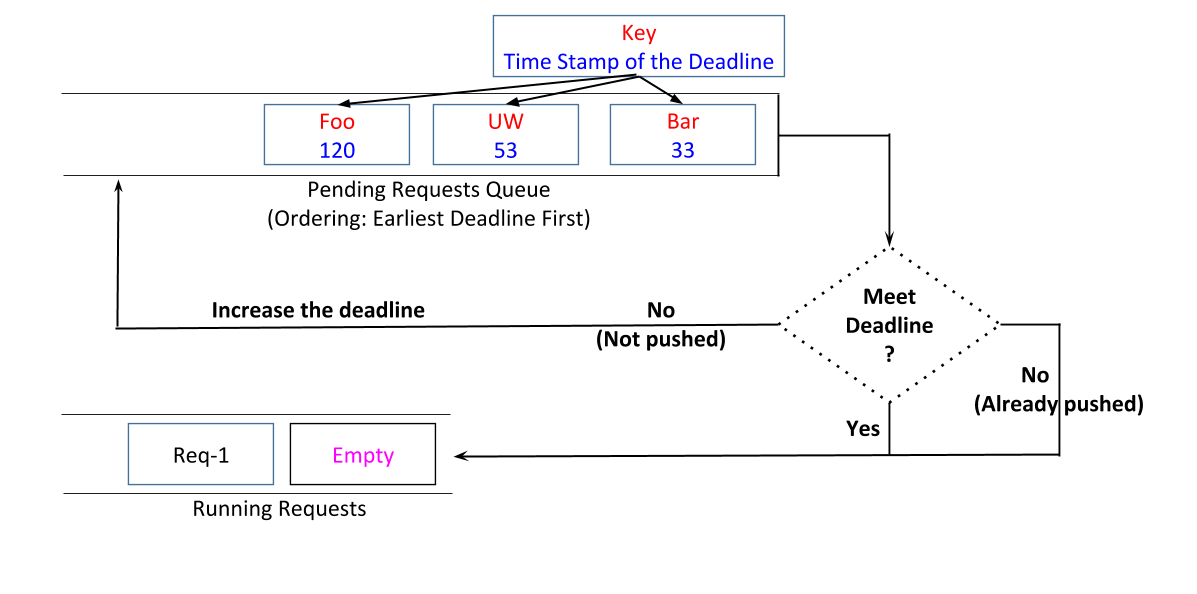
\includegraphics[scale=0.33]{img/DLS_Example8_4.png}}
    \end{center}
  \end{figure}
\end{frame}

\begin{frame}
  \frametitle{DLS - An Example (11)}
  \begin{itemize}
  \item DLS informs the client that the wait is over.
\newline
  \end{itemize}
  \begin{figure}
    \begin{center}
      \centerline{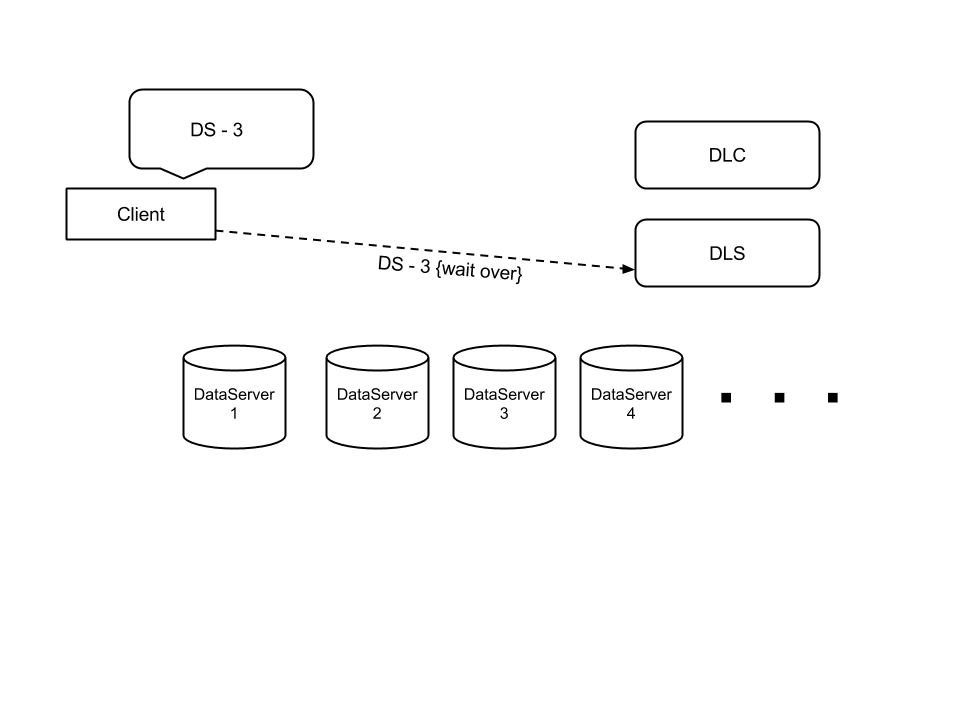
\includegraphics[scale=0.35]{img/DLS_Example10.png}}
    \end{center}
  \end{figure}
\end{frame}


\begin{frame}
  \frametitle{DLS - An Example (12)}
  \begin{itemize}
  \item The clients issues the read request to the data server.
\newline
  \end{itemize}
  \begin{figure}
    \begin{center}
      \centerline{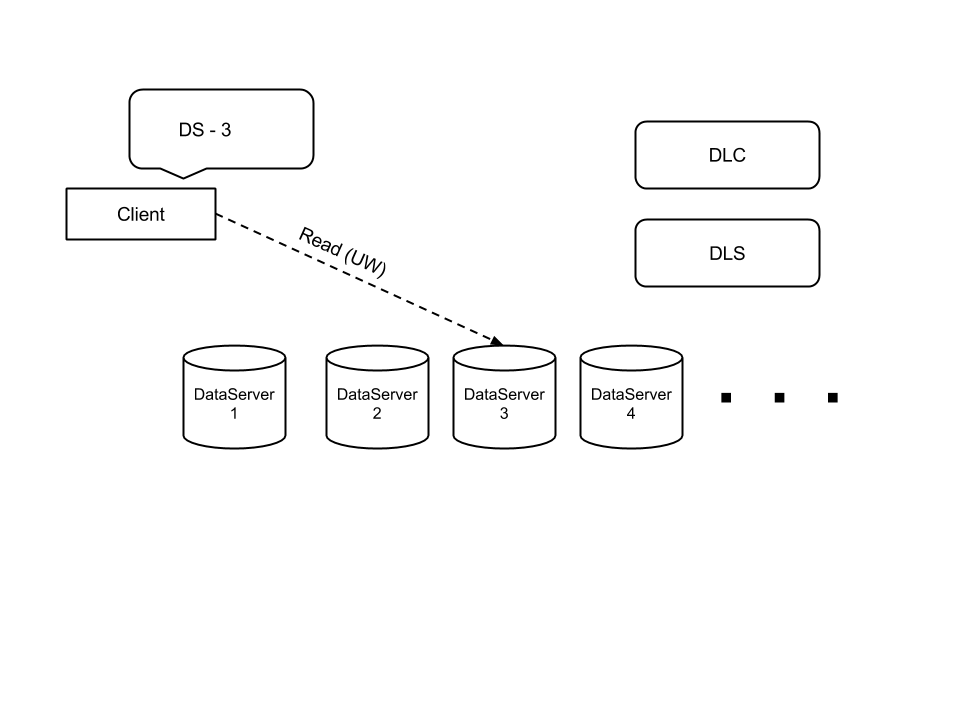
\includegraphics[scale=0.35]{img/DLS_Example11.png}}
    \end{center}
  \end{figure}
\end{frame}

\begin{frame}
  \frametitle{DLS - An Example (13)}
  \begin{itemize}
  \item After receiving the response, the client releases
    the ticket and concurrently inserts the data into the cache.
  \end{itemize}
  \begin{figure}
    \begin{center}
      \centerline{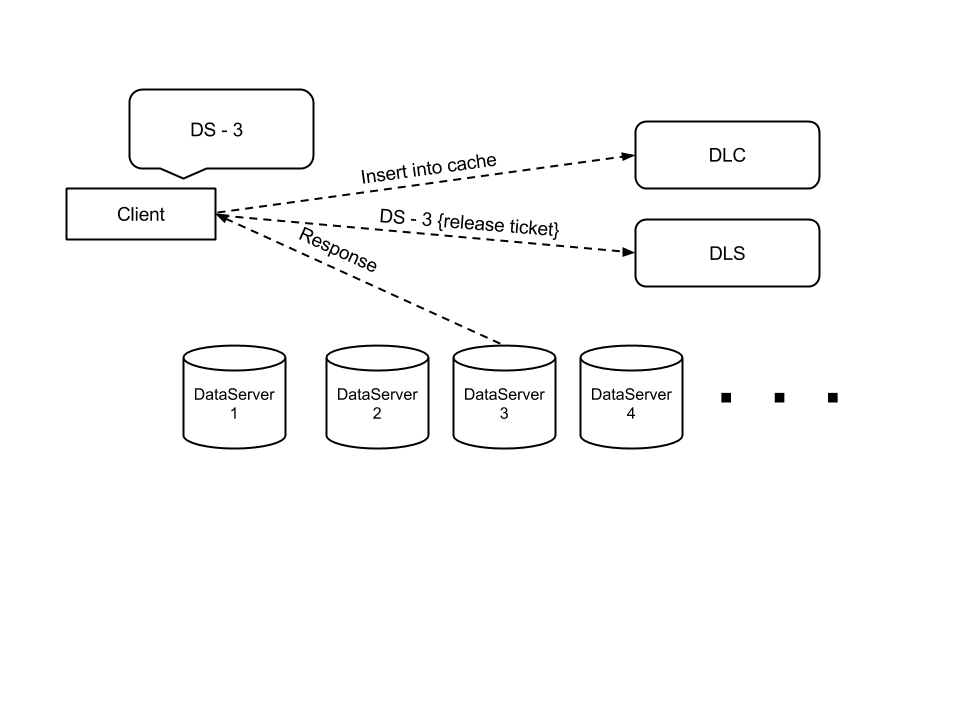
\includegraphics[scale=0.35]{img/DLS_Example12.png}}
    \end{center}
  \end{figure}
\end{frame}


\begin{frame}
  \frametitle{DLS - Admission Control}
  \begin{itemize}
  \item Bound the fraction of requests that miss their deadlines.
  \item Requests are rejected in two situations.
    \begin{itemize}
    \item The request will be miss its own deadline.
    \item The new request will cause already accepted requests to miss their deadlines.
    \end{itemize}
  \item Provides a system parameter $\beta$ as a knob to control the percentage
    of deadline misses.
  \end{itemize}
\end{frame}

\begin{frame}
  \frametitle{Full MicroFuge}
  \begin{itemize}
  \item
    MicroFuge combines both the DLC and DLS layers to achieve its best
    performance.
  \end{itemize}
  \begin{figure}
    \begin{center}
      \centerline{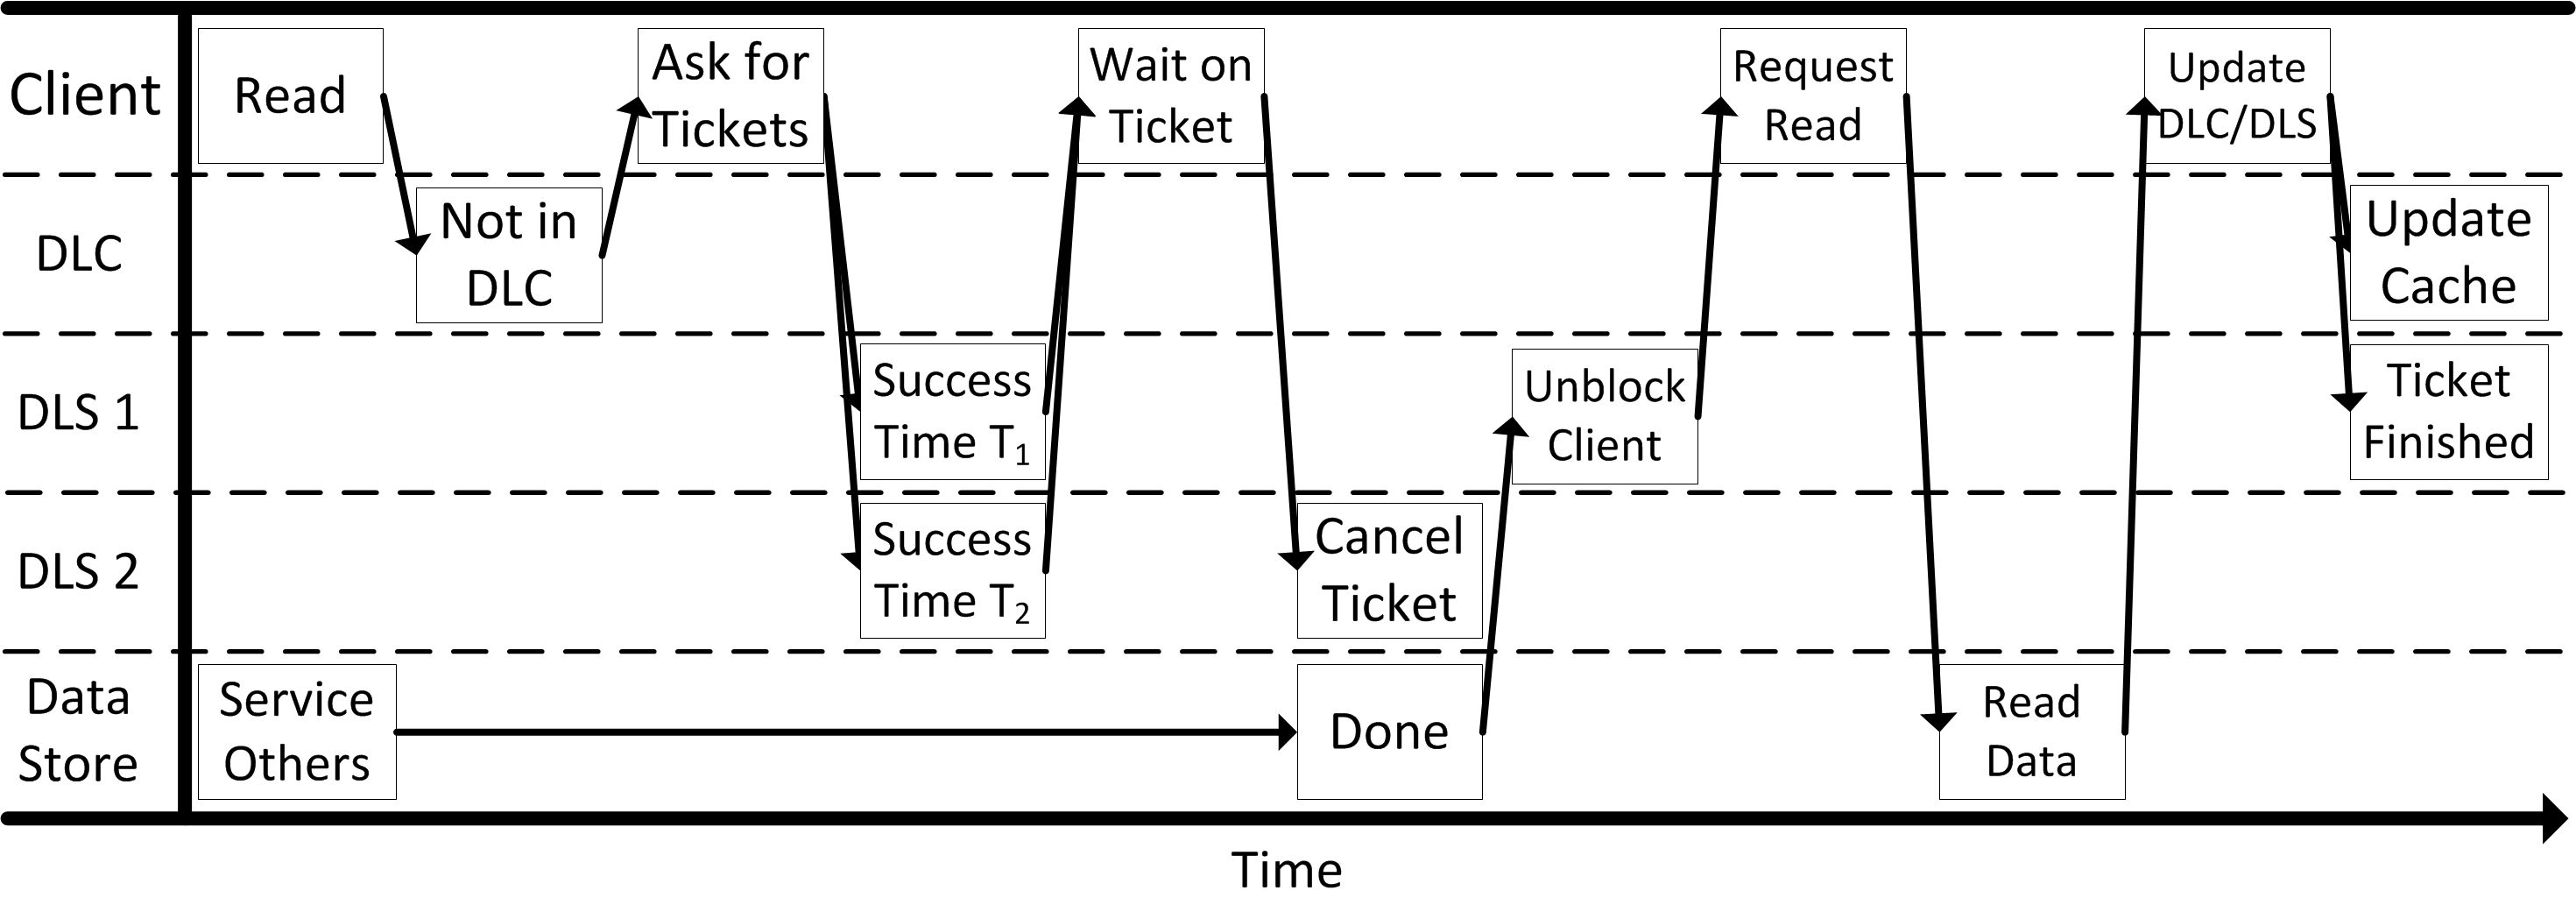
\includegraphics[scale=0.60]{img/RequestTimelineHorizontal.png}}
    \end{center}
  \end{figure}
\end {frame}



%% \begin{frame}
  %% \frametitle{Goals of the Evaluation}
  %% \begin{itemize}
  %% \item Comparison of the two caching systems.
    %% \begin{itemize}
    %% \item Deadline Cache
    %% \item Memcached
    %% \end{itemize}
  %% \item Effectiveness of MicroFuge.
    %% \begin{itemize}
    %% \item Caching Layer
    %% \item Scheduling layer
    %% \item Admission control
    %% \end{itemize}
  %% \end{itemize}
%% \end{frame}


\begin{frame}
  \frametitle{Experimental Setup - The Cluster}
  \begin{itemize}
  \item Twenty-node test cluster on AWS. Each cluster node is an m1.medium
    EC2 instance.
  \end{itemize}
  \begin{figure}
    \begin{center}
      \centerline{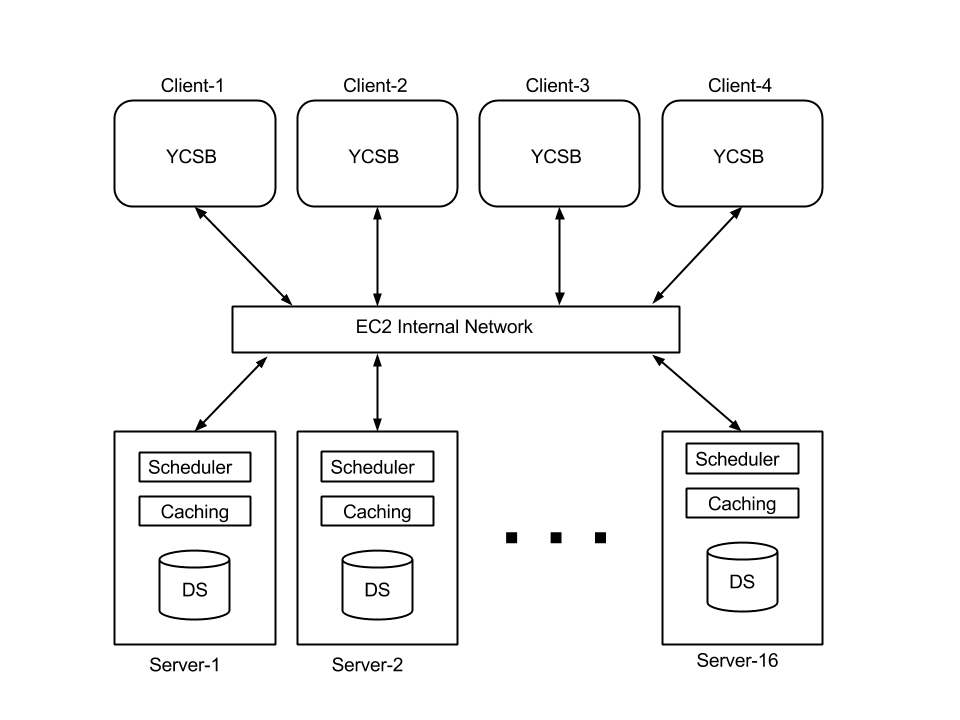
\includegraphics[scale=0.25]{img/Experimental_Setup.png}}
    \end{center}
  \end{figure}
\end{frame}

\begin{frame}
  \frametitle{Experimental Setup - Details}
  \begin{itemize}
  \item DataServer - Simple key-value store that uses leveldb with a
    replication factor of 3.
  \item Benchmarking System - Modified version of Yahoo! Cloud Serving
    Benchmark (YCSB).
    \begin{itemize}
    \item Assign deadlines to each key.\\
      %% \begin{center}
      \begin{tabular}{| l | c |}
        \hline
        Range & Percentage \\ \hline
        10-30ms & 20\% \\ \hline
        30-100ms & 30\% \\ \hline
        100-1000ms & 50\% \\ \hline
      \end{tabular}
      %% \end{center}
    \end{itemize}
  \item Data Set - Key-value store with 80 million records, 86.4 GB in size.
  \item Cache - Total capacity of 19.2GB.
  \end{itemize}
  % NOTES: We selected one range of deadlines which looked reasonable to us.
\end{frame}


\begin{frame}
  \frametitle{Deadline-Aware Caching with DLC}
  \begin{figure}[t]
    \begin{center}
      \centerline{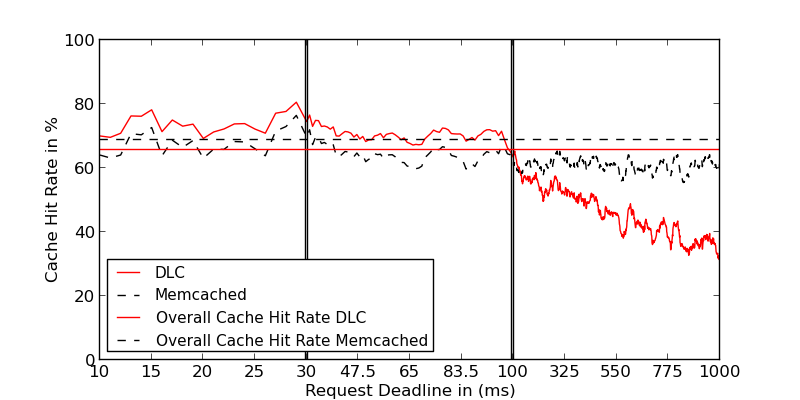
\includegraphics[scale=0.5]{img/EC2/EC2_CS_MM/cache_48.png}}
      \caption{Cache hit rate for 192 concurrent clients with DLC and Memcached.}
      \label{fig:cache_192_cs_mm}
    \end{center}
  \end{figure}
\end{frame}

\begin{frame}
  \frametitle{Deadline-Aware Caching with DLC and DLS}
  \begin{figure}[t]
    \begin{center}
      \centerline{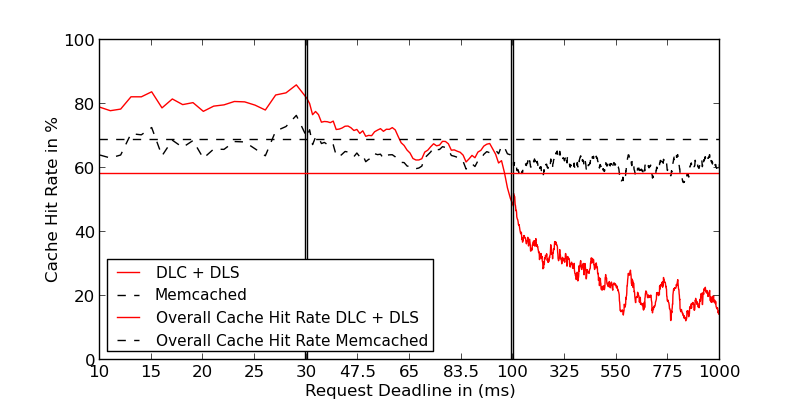
\includegraphics[scale=0.5]{img/EC2/EC2_SH_MM/cache_48.png}}
      \caption{Cache hit rate for 192 concurrent clients with DLC + DLS and Memcached.}
      \label{fig:cache_192_sh_mm}
    \end{center}
  \end{figure}
\end{frame}

\begin{frame}
  \frametitle{Deadline Miss Rate with DLC}
  \begin{figure}[t]
    \begin{center}
      \centerline{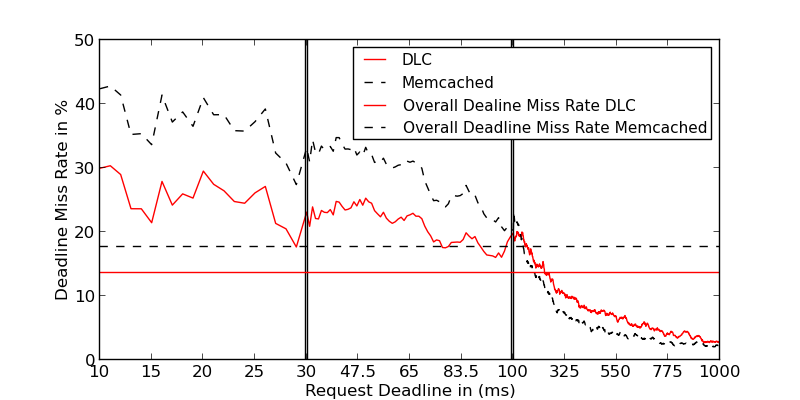
\includegraphics[scale=0.5]{img/EC2/EC2_CS_MM/miss_48.png}}
      \caption{Deadline miss rate for 192 concurrent clients with DLC and Memcached.}
      \label{fig:miss_192_cs_mm}
    \end{center}
  \end{figure}
\end{frame}


\begin{frame}
  \frametitle{Deadline Miss Rate with DLC and DLS}
  \begin{figure}[t]
    \begin{center}
      \centerline{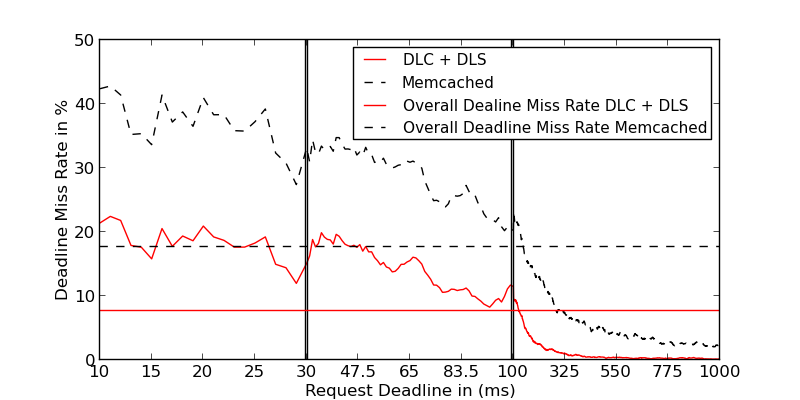
\includegraphics[scale=0.5]{img/EC2/EC2_SH_MM/miss_48.png}}
      \caption{Deadline miss rate for 192 concurrent clients with DLC + DLS and Memcached.}
      \label{fig:miss_192_sh_mm}
    \end{center}
  \end{figure}
\end{frame}

%% \begin{frame}
  %% \frametitle{Experimental Results - Deadline Miss 3}
  %% \begin{figure}[t]
    %% \begin{center}
      %% \centerline{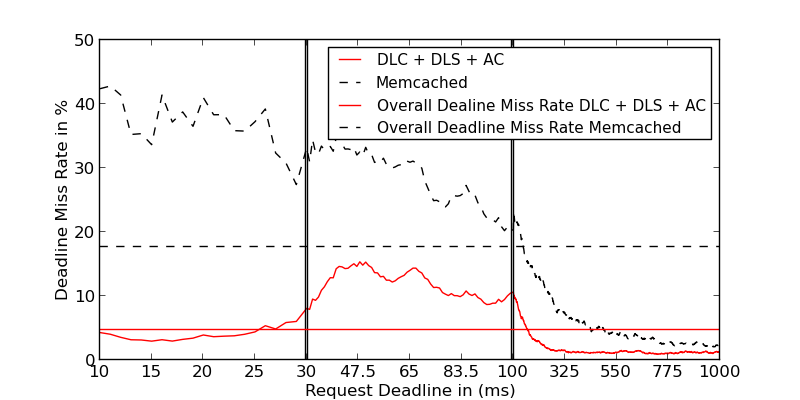
\includegraphics[scale=0.5]{img/EC2/EC2_AC_MM/miss_48.png}}
      %% \caption{Deadline miss rate for 192 concurrent clients with DLC + DLS + AC and Memcached.}
      %% \label{fig:miss_192_ac_mm}
    %% \end{center}
  %% \end{figure}
%% \end{frame}

%% \begin{frame}
  %% \frametitle{Experimental Results - Tunable Admission Control}
  %% \begin{figure}[t]
    %% \begin{center}
      %% \centerline{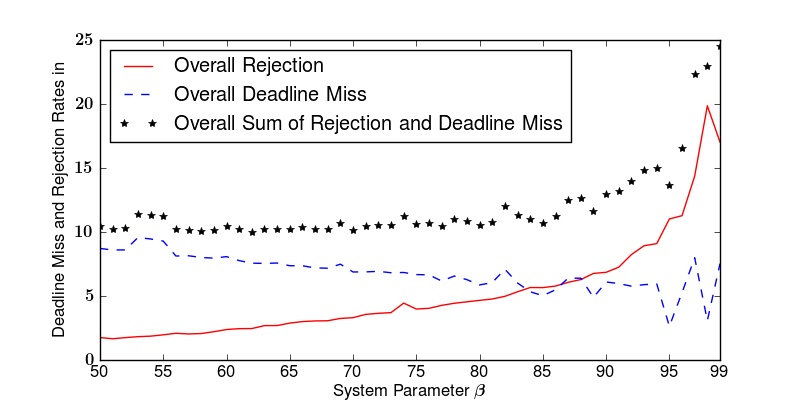
\includegraphics[scale=0.5]{img/EC2/Varying_ac/varying_acPerc_192.png}}
      %% \caption{Deadline miss vs. rejection rates with respect to various values of
        %% system parameter $\beta$ for 192 clients.}
      %% \label{fig:varying_ac}
    %% \end{center}
  %% \end{figure}
%% \end{frame}

\begin{frame}
  \frametitle{Conclusion}
  \begin{itemize}
  \item Predictable performance is necessary in multi-tenant environments.
  \item MicroFuge tackles the performance isolation problem with its
    deadline-aware caching and scheduling middleware.
  \item MicroFuge reduces deadline miss rate from over 20\% to
    less than 5\%.
  \end{itemize}
\end{frame}
\end{document}
